\documentclass[12pt, a4paper]{article}
\usepackage[utf8]{inputenc}
\usepackage[T1]{fontenc}
\usepackage{lmodern}

\usepackage[spanish,es-noshorthands]{babel}

\usepackage{amsmath,amssymb,amsthm}
\usepackage{amsfonts}
\usepackage{authblk}
\usepackage{mathtools}

\usepackage{graphicx}
\graphicspath{{Images/}}
\usepackage{float}
\usepackage{fullpage}
\parskip = 2pt plus 1.5pt minus 1pt
\usepackage{tikz}
\usetikzlibrary{positioning}
\usetikzlibrary{babel}
\pgfdeclarelayer{background}
\pgfdeclarelayer{foreground}
\pgfsetlayers{background,main,foreground}

\numberwithin{equation}{section}

\theoremstyle{definition}
\newtheorem{defi}{Definición}
\newtheorem{ejemplo}{Ejemplo}
\newenvironment{ejem}
  {\pushQED{\qed}\renewcommand{\qedsymbol}{$\blacktriangleleft$}\ejemplo}
  {\popQED\endejemplo}

\theoremstyle{remark}
\newtheorem*{remark}{Nota}

\theoremstyle{plain}
\newtheorem{prop}{Proposición}

\title{Sobre la homología persistente en redes neuronales}


\author{José Manuel Ros Rodrigo}

\affil{Facultad de Ciencia y Tecnología\\
  Universidad de La Rioja}

\date{Marzo 2022}

\begin{document}
	
	\maketitle
	
	\newpage
	
	\begin{abstract}
	(En construcción.)
	\end{abstract}
	
	\newpage

	\tableofcontents

	\newpage

	\section{Introducción}
	(En construcción.)

	\newpage

	\section{Preeliminares}

	A lo largo de este capítulo vamos a ver todas las nociones teóricas 
	necesarias para el uso de la homología persistente en redes neuronales.	
	
	\subsection{Complejos simpliciales}
	Comenzamos con el primer concepto fundamental de todo el trabajo, los 
	\emph{complejos simpliciales}. Esta noción admite dos enfoques 
	diferentes, por lo que debemos dintinguir entre dos definiciones 
	equivalentes: los complejos simpliciales \emph{abstractos} y los 
	complejos simpliciales \emph{geométricos}.

	Siguiendo el enfoque combinatorio, comenzamos definiendo los complejos 
	simpliciales abstractos y algunas nociones relacionadas. 

	\begin{defi}
	
	Un \textit{complejo simplicial abstracto} es una colección, 
	\begin{Large}$\nu$\end{Large}, de subconjuntos no vacíos de un 
	conjunto, {\Large $\nu$}$_{0}$, que verifica las siguientes 
	propiedades:
	
	\begin{enumerate}
		\item Si $v \in $ {\Large $ \nu$}$_{0}$, entonces $\{v\} \in$
			\begin{Large}$ \nu$\end{Large}
		\item Si $\sigma \in $ {\Large $ \nu$}$ \text{ y } \tau 
			\subset \sigma$, entonces $ \tau \in $
			\begin{Large}$ \nu$\end{Large}
	\end{enumerate}
	
	A los elementos de {\Large $\nu$} los llamaremos \textit{símplices},
	más concretamente: dado $\sigma \in $ {\Large $\nu$}, diremos que 
	$\sigma$ tiene \textit{dimensión p}, y que $\sigma$ es un 
	\textit{p-símplice}, si $|\sigma|=p+1$. Asimismo, definimos la 
	\textit{dimensión de {\Large $\nu$}} como el máximo de las dimensiones 
	de sus símplices y denotaremos por {\Large $\nu$}$_{p}$ a la colección 
	de los p-símplices de {\Large $\nu$}.	
	
	\end{defi}
	
	En relación con el concepto de símplice y de dimensión surge la 
	siguiente noción: 

	\begin{defi}
		Sean $\sigma$ y $\tau$ dos símplices de {\Large $\nu$} tales 
		que $\tau \subset \sigma$. Entonces diremos que $\tau$ es una 
		\textit{cara} de $\sigma$, y si las dimensiones de $\sigma$ y 
		$\tau$ difieren por a, diremos que $\tau$ es una cara de 
		$\sigma$ de \textit{codimensión a}.
	\end{defi}

	Ahora que hemos definido los complejos simpliciales abstractos veamos 
	un pequeño ejemplo para fijar ideas.

	\begin{ejem}
		Supongamos el siguiente complejo simplicial abstracto:
		\begin{multline*} 
			\text{{\Large $\nu$}}=\{\{a\},\{b\},\{c\},\{d\},
			\{a,b\},\{a,c\},\{a,d\},\{b,c\},\{b,d\},\{c,d\},
			\{a,b,c\},\{a,b,d\},\\
			\{a,c,d\},\{a,b,c,d\}\}
		\end{multline*}
		Así, tenemos que la dimensión de {\Large $\nu$} es 3. También 
		observamos que el 3-símplice $\{a,b,c,d\}$ tiene por caras de 
		codimensión 1 a los 2-símplices $\{a,b,c\},\{a,b,d\}$ y 
		$\{a,c,d\}$. Veamos su representación geométrica.

		\begin{figure}[H]
			\centering
			\begin{tikzpicture}
				%Nodes
				\coordinate      (a) 	at 	(4.5,2.5);
				\coordinate      (b) 	at 	(3,0.8);
				\coordinate     (c) 	at 	(4.4,0.1);
				\coordinate      (d) 	at 	(6,0.8);
				
				%Lines
		    		\draw[thick, fill=black!20] (a) -- (b) -- (c) -- (d) -- cycle;
				\draw[thick, dashed] (b) -- (d);
				\draw[thick] (a) -- (c);

				\fill[black!20, draw=black, thick] (a) circle (3pt) node[black, above right] {a};
				\fill[black!20, draw=black, thick] (b) circle (3pt) node[black, above left] {b};
				\fill[black!20, draw=black, thick] (c) circle (3pt) node[black, below right] {c};
				\fill[black!20, draw=black, thick] (d) circle (3pt) node[black, above right] {d};

			\end{tikzpicture}
			\caption{Representación geométrica del complejo 
			simplicial {\Large $\nu$}.}
		\end{figure}

		Esta representación es única salvo homeomorfismo. Observamos 
		que interpretando {\Large $\nu$} como un subconjunto de 
		$\mathbb{R}^{n}$ obtenemos un tetraedro. Esta idea motiva el 
		otro enfoque de los complejos simpliciales: el enfoque 
		geométrico.
	\end{ejem}

	Siguiendo el enfoque geométrico es necesario que, antes de llegar a la
	definición de complejo simplicial geométrico, veamos unos conceptos 
	previos relacionados con la propia definición.

	\begin{defi}
		Sean $\{u_{0},u_{1},...,u_{k}\}\subset\mathbb{R}^{n}$. Diremos
		que los k+1 puntos son \textit{afínmente independientes} si 
		los k vectores $u_{1}-u_{0},u_{2}-u_{0},...,u_{k}-u_{0}$ son
		linealmente independientes.

		Sea $x \in \mathbb{R}^{n}$. Diremos que $x$ es una 
		\textit{combinación afín} de los $u_{i}$ si $\exists 
		\lambda_{0},...,\lambda_{k}$ tales que 
		$x=\sum_{i=0}^{k}\lambda_{i}u_{i}$ y 
		$\sum_{i=0}^{k}\lambda_{i}=1$
	\end{defi}

	\begin{defi}
		Sean $\{u_{0},u_{1},...,u_{k}\}\subset\mathbb{R}^{n}$ k+1 
		puntos afínmente independientes y $x=\sum_{i=0}^{k}
		\lambda_{i}u_{i}$ una combinación afín. Diremos que $x$ es una
		\textit{combinación convexa} de los $u_{i}$ si todos los 
		$\lambda_{i}$ son no negativos.

		Definimos la \textit{clausura convexa} de los $u_{i}$ como el
		conjunto de todas sus posibles combinaciones convexas.
	\end{defi}

	Ahora que ya contamos con estas nociones previas pasamos a definir la 
	pieza clave en la definición de complejo simplicial geométrico: el 
	\emph{símplice}.

	\begin{defi}
		Definimos un \textit{k-símplice} como la clausura convexa de 
		k+1 puntos afínmente independientes. Lo denotaremos por 
		$\sigma=conv\{u_{0},u_{1},...,u_{k}\}$, y diremos que la 
		\textit{dimensión de $\sigma$} es k.

		Llamamos \textit{cara} de $\sigma$ a cualquier combinación 
		convexa de un subconjunto no vacío de los $u_{i}$. Lo 
		denotaremos por $\leq$.

		Para los casos $k=0,1,2,3$ diremos que $\sigma$ es un vértice,
		arista, triángulo, tetraedro respectivamente.
	\end{defi}

	Habiendo definido todos los conceptos previos necesarios pasamos a 
	definir \emph{complejo simplicial geométrico}.

	\begin{defi}
		Llamamos \textit{complejo simplicial geométrico} a la 
		colección finita de símplices {\Large $\nu$} verificando las
		siguientes propiedades:
		\begin{enumerate}
			\item Si $\sigma\in \text{{\Large $\nu$} y }
				\tau \leq \sigma \implies \tau \in 
				\text{{\Large $\nu$}}$
			\item Si $\sigma_{1},\sigma_{2} \in 
				\text{{\Large $\nu$}} \implies 
				\sigma_{1}\cap\sigma_{2}=\emptyset \text{ o }
				\sigma_{1}\cap\sigma_{2} \text{ es una cara 
				común a ambos.}$
		\end{enumerate}
	\end{defi}
	
	De aquí en adelante emplearemos la definición de complejo simplicial 
	abstracto, pues es la más adecuada para el presente trabajo.

	Ahora que ya hemos definido los objetos con los que vamos a trabajar, 
	procedemos a definir las aplicaciones entre ellos.
	\begin{defi}
		Una \textit{aplicación entre complejos simpliciales}, 
		$f:\text{{\Large $\nu$}} \rightarrow \text{{\Large 
		$\nu$}$^{\prime}$}$, es una aplicación $f:\text{{\Large 
		$\nu$}$_{0}$} \rightarrow \text{{\Large $\nu$}$_{0}^{\prime}$}$ 
		tal que $f(\sigma) \in \text{{\Large $\nu$}$^{\prime}$} 
		\hspace{5pt} \forall \sigma \in \text{{\Large $\nu$}}$.
	\end{defi}
	
	Teniendo definidas las aplicaciones entre complejos simpliciales, 
	vamos a dotar a los complejos simpliciales de una cierta estructura 
	que será de lo más útil para los propósitos del presente trabajo.

	Consideremos $\mathbb{Z}_{2}$ el cuerpo de dos elementos. Dado un 
	complejo simplicial {\Large $\nu$}, denotaremos por 
	$C_{p}(\text{{\Large $\nu$}})$ al $\mathbb{Z}_{2}$-espacio vectorial
	libre cuya base viene dada por los p-símplices de {\Large $\nu$}. 
	Ahora, para cualquier $p \in \{1,2,...\}$ definimos la siguiente 
	aplicación: 
	\begin{equation}
		\label{def:borde}
		\begin{array}{lll}
			\partial_{p}:C_{p}(\text{{\Large $\nu$}}) & 
				\rightarrow & C_{p-1}(\text{{\Large $\nu$}})
				\\[3pt] 
			\multicolumn{1}{r}{c} & \mapsto & \displaystyle 
				\sum_{\mathclap{d \subset c,d \in 
				\text{{\large $\nu$}}_{p-1}}}d
		\end{array} 
	\end{equation}
	Si $p=0$ definimos $\partial_{0}=0$. Intuitivamente, $\partial_{p}$ le
	asigna a cada p-símplice su borde, esto es, la suma de sus caras de
	codimensión 1. Esta aplicación tiene una propiedad muy importante, 
	que motivará la siguiente subsección:

	\begin{prop}
		Sea $\partial_{p}$ definida como en \ref{def:borde}. Entonces 
		para todo $p \in \{0,1,2,..\}$ $\partial_{p}\circ 
		\partial_{p+1}=0$. Coloquialmente, <<el borde del borde es 
		vacío>>.
	\end{prop}
	\begin{proof}
		Sea $c \in C_{p+1}(\text{{\Large $\nu$}})\text{ y }v\in 
		\text{{\Large $\nu$}}$ el símplice representado por $c$. 
		Veamos que $\partial_{p}(\partial_{p+1}(c))=0$.

		En efecto, notemos que $v$ posee $\binom{p+2}{p}$ 
		caras distintas de codimensión 2. Sea $\tau$ una de ellas, es 
		decir, $\tau$ es un p-1-símplice y $\tau \subset v$.

		Si probamos que $\tau$ aparece en 2 caras de codimensión 1 de 
		$v$ habremos terminado, pues aparecerá 2 veces como vector al 
		hacer $\partial_{p}(\partial_{p+1}(c))$ y como estamos en 
		$\mathbb{Z}_{2}$ se anulará. Esto implica lo que queremos
		probar.

		Observemos que $\tau$ tiene dimensión p mientras que $v$ tiene
		dimensión p+2. Por lo tanto, supongamos, sin pérdida de 
		generalidad, que $\tau$ viene dado por los p últimos elementos 
		de $v$. Así, tenemos dos elementos libres en $v$, y al 
		calcular las caras de codimensión 1 de $v$, con los p últimos 
		elementos fijos, tendremos únicamente 2 caras que contienen a
		$\tau$.  	
	\end{proof}
	\begin{remark}
		La elección del cuerpo sobre el que se toman los espacios 
		vectoriales es muy significativa. De hecho, si escogemos otro 
		cuerpo, los resultados serán muy distintos, y los cálculos 
		para llegar a ellos, serán más engorrosos.
	\end{remark}

	Veamos un pequeño ejemplo que ilustre esta nota.

	\begin{ejem}
		Supongamos el complejo simplicial {\Large $\nu$} del ejemplo 
		anterior. 
	\end{ejem}

	De la proposición anterior se desprende que $Im(\partial_{p+1}) 
	\subset Ker(\partial_{p})$. Este hecho motiva la siguiente noción 
	importante del presente trabajo: los \emph{grupos de homología}.
 

	\subsection{Homología. Homología persistente}
	
	En la subsección anterior, más concretamente en \ref{def:borde}, hemos 
	introducido la aplicación <<borde>>. A lo largo de esta subsección 
	vamos a profundizar más en ella, y en los espacios sobre los que está
	definida, llegando de una manera natural a la definición de 
	\emph{grupo de homología}.

	En primer lugar, vamos a centrarnos en 
	$C_{p}(\text{{\Large $\nu$}})$ y sus elementos.

	Tal y como hemos mencionado anteriormente, podemos ver 
	$C_{p}(\text{{\Large $\nu$}})$ como un $\mathbb{Z}_{2}$-espacio 
	vectorial libre cuya base viene dada por los p-símplices de 
	{\Large $\nu$}. Así, si $c \in C_{p}(\text{{\Large $\nu$}})$, entonces
	$c$ es un vector que representa a un p-símplice $v$. De esta manera,
	podemos ver $v$ como suma de los p-símplices de las componentes no 
	nulas de $c$. Más formalmente:

	\begin{defi}
		Sea {\Large $\nu$} un complejo simplicial y $p \in \mathbb{N}
		\cup\{0\}$ 
		tal que $p\leq dim \text{{\Large $\nu$}}$. Una 
		\textit{p-cadena} es una suma formal de p-símplices de 
		{\Large $\nu$}.
	\end{defi}
	
	Con la noción de p-cadena, ya podemos formalizar la definición de 
	$C_{p}(\text{{\Large $\nu$}})$. 

	\begin{defi}
		Sea {\Large $\nu$} un complejo simplicial abstracto. Definimos
		el \textit{grupo de p-cadenas} de {\Large $\nu$} como el 
		conjunto de todas las p-cadenas de 
		{\Large $\nu$}, con la operación suma componente a componente 
		con coeficientes en $\mathbb{Z}_{2}$. Lo denotaremos por 
		$(C_{p}(\text{{\Large $\nu$}}), +)$ o simplemente 
		$C_{p}(\text{{\Large $\nu$}})$.
	\end{defi}

	De la definición anterior se desprende el siguiente resultado:

	\begin{prop}
		\label{prop:abel}
		Sea {\Large $\nu$} un complejo simplicial abstracto. Para cada 
		$p \in \mathbb{N}\cup\{0\}$ tal que $p \leq dim\text{{\Large $\nu$}}$, 
		entonces $(C_{p}(\text{{\Large $\nu$}}), +)$ es grupo 
		abeliano.
	\end{prop}

	\begin{proof}
		La asociatividad se tiene por herencia de la suma en 
		$\mathbb{Z}_{2}$. La existencia de elemento neutro es clara, 
		pues bastará considerar el vector nulo. La existencia de 
		opuesto también es inmediata, ya que todo elemento es opuesto 
		de sí mismo. Finalmente, como la suma en $\mathbb{Z}_{2}$ es 
		conmutativa, se sigue que $(C_{p}(\text{{\Large $\nu$}}), +)$
		es abeliano.
	\end{proof}

	En segundo lugar, y habiendo definido los grupos de p-cadenas, pasamos
	a hacer un estudio más detallado de la aplicación <<borde>> definida 
	en \ref{def:borde}. Vamos con su definición:

	\begin{defi}
		Sea {\Large $\nu$} un complejo simplicial abstracto, $\sigma 
		\in \text{{\Large $\nu$}}$ y $\sigma = \{u_{1},...,u_{p}\}$. 
		Definimos el \textit{homomorfismo borde} para un símplice 
		como:
		$$
		\partial_{p}(\sigma)=\displaystyle 
		\sum_{j=0}^{p}\{u_{1},...,\widehat{u_{j}},...,u_{p}\}
		$$
 		Donde $\widehat{u_{j}}$ indica que omitimos $u_{j}$. Además,
		podemos extender esta definición para cadenas, en concreto:
	\begin{equation}
		\label{def:borde_form}
		\begin{array}{lll}
			\partial_{p}:C_{p}(\text{{\Large $\nu$}}) & 
				\rightarrow & C_{p-1}(\text{{\Large $\nu$}})
				\\[3pt] 
			\multicolumn{1}{r}{c=\sum\sigma_{i}} & \mapsto & 
			\partial_{p}(c)=\sum\partial_{p}(\sigma_{i})
		\end{array}
	\end{equation}
	A los elementos de $Im(\partial_{p})$ los llamaremos 
	\textit{(p-1)-bordes}, y a los elementos de $Ker(\partial_{p})$, 
	\textit{p-ciclos}.
	\end{defi}
	\begin{proof}
		Vamos a probar que $\partial_{p}$ es, en efecto, un 
		homomorfismo.

		Sean $\sigma,\tau \in \text{{\Large $\nu$}}_{p}$ tales que
		$\sigma = \{u_{1},...,u_{p}\}$ y $\tau = \{w_{1},...,w_{p}\}$.

		$\partial_{p}(\sigma)+\partial_{p}(\tau)=\displaystyle 
		\sum_{j=0}^{p}\{u_{1},...,\widehat{u_{j}},...,u_{p}\} + 
		\displaystyle \sum_{j=0}^{p}\{w_{1},...,\widehat{w_{j}},...,
		w_{p}\}=\displaystyle \sum_{i=0}^{p}\sum_{j=0}^{p}\{u_{1} + 
		w_{1},...,\widehat{u_{i}} + \widehat{w_{j}},...,u_{p}+w_{p}\}=
		\partial_{p}(\sigma+\tau)$. 

		Esto prueba que $\partial_{p}$ conmuta con la suma para 
		símplices. Como conmuta para símplices, se sigue que conmuta 
		para cadenas.

		Ahora, $0=\partial_{p}(\sigma)+\partial_{p}(\sigma)=
		\partial_{p}(\sigma + \sigma)=\partial_{p}(0)$. Esto implica 
		que $\partial_{p}$ deja fijo el símplice neutro. Al igual que
		antes, esta propiedad se extiende para cadenas.

		Finalmente, $0=\partial_{p}(0)=\partial_{p}(\sigma - \sigma)=
		\partial_{p}(\sigma)+\partial_{p}(-\sigma)$ y sumando 
		$-\partial_{p}(\sigma)$ a ambos lados de la ecuacion se sigue 
		que $\partial_{p}$ conmuta con el opuesto. Una vez más, este 
		hecho se extiende a cadenas.
	\end{proof}

	Este homomorfismo tiene propiedades muy interesantes, entre ellas:

	\begin{prop}
		Sea $\partial_{p}$ el homomorfismo borde definido en 
	   	\ref{def:borde_form}. Entonces $Im(\partial_{p})$ es subgrupo 
		de $C_{p-1}(\text{{\Large $\nu$}})$ y $Ker(\partial_{p})$ es 
		subgrupo de $C_{p}(\text{{\Large $\nu$}})$. Más aún, ambos son
		subgrupos normales de $C_{p-1}(\text{{\Large $\nu$}})$, 
		$C_{p-1}(\text{{\Large $\nu$}})$ respectivamente.
	\end{prop}
	\begin{proof}
		Vamos a probar ambos hechos por separado:
		\begin{itemize}
			\item Probaremos primero que $Im(\partial_{p})$ es subgrupo:

			Sean $a,b \in Im(\partial_{p})$ tales que $a=\partial_{p}(c) 
			\text{ y } b=\partial_{p}(d), c,d \in 
			C_{p}(\text{{\Large $\nu$}})$. 

			Entonces $a+b=\partial_{p}(c)+\partial_{p}(d)=
			\partial_{p}(c+d)$. Esto implica que $Im(\partial_{p})$ es 
			cerrado para la suma.

			Ahora, $0=\partial_{p}(0)=\partial_{p}(c+c)=
			\partial_{p}(c)+\partial_{p}(c)=a+a$. Esto implica que 
			$Im(\partial_{p})$ es cerrado para opuestos.

			Se sigue que $Im(\partial_{p})\leq 
			C_{p-1}(\text{{\Large $\nu$}})$.
			
			\item Probemos ahora que $Ker(\partial_{p})$ es 
			subgrupo: 
				
			Al igual que antes, sean $a,b \in Ker(\partial_{p})$.

			Entonces $0=\partial_{p}(a)+\partial_{p}(b)=
			\partial_{p}(a+b)$. Esto prueba que 
			$Ker(\partial_{p})$ es cerrado para la suma.

			Ahora, $0=\partial_{p}(0)=\partial_{p}(a-a)=
			\partial_{p}(a)+\partial_{p}(-a)=\partial_{p}(-a)$. 
			Esto prueba que $Ker(\partial_{p})$ es cerrado para 
			opuestos.

			Se sigue que $Ker(\partial_{p})\leq 
			C_{p}(\text{{\Large $\nu$}})$.
		\end{itemize}
		En virtud de la proposición \ref{prop:abel} y lo ya probado, 
		se concluye la normalidad.
	\end{proof}

	

	Además de la propiedad anterior, y tal y como vimos en la subsección 
	anterior, el homomorfismo borde tiene la propiedad fundamental de que 
	$\partial_{p}\circ \partial_{p+1}=0$. Este hecho implica que 
	$Im(\partial_{p+1}) \subset Ker(\partial_{p})$. Por lo tanto, podemos 
	considerar el cociente entre ambos grupos: $Ker(\partial_{p})/
	Im(\partial_{p+1})$. Este cociente constituye una de las piezas clave
	del presente trabajo:

	\begin{defi}
		\label{defi:homology}
		Sea $p \in \mathbb{N}\cup\{0\}$ y {\Large $\nu$} un complejo 
		simplicial. Definimos el \textit{p-ésimo grupo de homología} 
		de {\Large $\nu$} como el grupo cociente $Ker(\partial_{p})/
		Im(\partial_{p+1})$, donde $\partial_{p}$ está definida como
		en \ref{def:borde_form}. Lo denotaremos por $H_{p}(\text{
		{\Large $\nu$}})$.

		A su cardinal, $|H_{p}(\text{{\Large $\nu$}})|=
		|Ker(\partial_{p})|-|Im(\partial_{p+1})|$, lo 
		llamaremos \textit{p-ésimo número de Betti}, y lo denotaremos
		por $\beta_{p}(\text{{\Large $\nu$}})$.
	\end{defi}

	Intuitivamente, los p-ciclos que no son p-bordes representan agujeros
	p-dimensionales. Por lo tanto, $\beta_{p}(\text{{\Large $\nu$}})$ 
	representa el número de p-agujeros de {\Large $\nu$}.

	\section{Nociones teóricas previas}
	
		Comenzamos dando algunas nociones básicas que nos serán muy útiles a lo largo del trabajo.
			
	\subsection{Homología}	

		Habiendo interiorizado los conceptos previos, vamos a usarlos en nuestros siguientes propósitos. Así pues, consideremos $\mathbb{F}_{2}$ el cuerpo de dos elementos. Dado un
		complejo simplicial {\Large $\nu$}, denotaremos por $C_{p}(\mathcal{K})$ al $\mathbb{F}_{2}$-espacio vectorial cuya base viene dada por los p-símplices de {\Large $\nu$}. Ahora,
		para cualquier $p \in \{1,2,...\}$ definimos la siguiente aplicación: 
		\begin{flalign*}
			& \left.
			\begin{array}{l}
				\partial_{p}:C_{p}(\mathcal{K}) \rightarrow C_{p-1}(\mathcal{K})\\[2pt] 
				\hspace{1.5cm} \sigma \mapsto \displaystyle \sum_{\mathclap{\tau \subset \sigma,\tau \in \mathcal{K}_{p-1}}}\tau
			\end{array}
			\right. &
		\end{flalign*}
		
		Si $p=0$ entonces definimos $\partial_{0}=0$. Observemos que $\partial_{p}$ le asigna a cada p-símplice su borde, esto es, la suma de sus caras de codimensión 1. Adicionalmente, podemos
		observar que $\forall p \in \{0,1,2,..\}$, $\partial_{p}\circ \partial_{p+1}=0$. De manera informal decimos que el borde del borde es vacío. Veamos un ejemplo para clarificar esta noción.

		\begin{ejem}
		
			Ejemplo conveniente de ''el borde del borde es vacío''. (En construcción).

		\end{ejem}

		De la observación anterior se desprende que $Im(\partial_{p+1}) \subset Ker(\partial_{p})$. Esta propiedad motiva la siguiente definición.
		\begin{defi}
			Sea $p \in \{0,1,...\}$. Definimos la \textit{p-ésima homología} de un complejo simplicial {\Large $\nu$} como el espacio vectorial cociente:	
			\begin{flalign*}
				& \left.
				H_{p}(\mathcal{K}):=Ker(\partial_{p})/Im(\partial_{p+1})
				\right. &
			\end{flalign*}
		\end{defi}

		\begin{remark}
			A la dimensión de $H_{p}(\mathcal{K})$ la denotaremos por $B_{p}(\mathcal{K}):=dim H_{p}(\mathcal{K})=dim Ker(\partial_{p})-dim Im(\partial_{p+1})$ y la llamaremos
			\textit{p-ésimo número de Betti}.\\
			A los elementos de $Im(\partial_{p+1})$ los llamaremos \textit{p-bordes}, y a los de $Ker(\partial_{p})$ \textit{p-ciclos}.
		\end{remark}

		De la anterior consideración, deducimos que el p-ésimo número de Betti representa el número de agujeros p-dimensionales de K. Además, si {\Large $\nu$} es un complejo simplicial
		de dimensión n, entonces $\forall p > n,\hspace{0.1cm} H_{p}(\mathcal{K})=0$ ya que $\mathcal{K}_{p}=\emptyset$. Esto nos lleva a la construcción de la siguiente cadena de 
		espacios vectoriales:
		\begin{flalign*}
			& \left.
			\begin{array}{l}
				\hspace{0.1cm} \partial_{n+1} \hspace{1.1cm} \partial_{n} \hspace{1.4cm} \partial_{n-1} \hspace{0.9cm} \partial_{2} \hspace{1.3cm} \partial_{1} \hspace{1.2cm} \partial_{0}\\
				0 \rightarrow C_{n}(\mathcal{K}) \rightarrow C_{n-1}(\mathcal{K}) \rightarrow \hspace{0.25cm} ... \hspace{0.25cm} \rightarrow C_{1}(\mathcal{K}) \rightarrow C_{0}(\mathcal{K}) \rightarrow 0
			\end{array}
			\right. &
		\end{flalign*}

		\begin{ejem}
			Ejemplo conveniente de homología simplicial. (En construcción).
		\end{ejem}	

	\subsection{Aplicaciones entre complejos simpliciales}

		Consideremos una aplicación entre complejos simpliciales, $f:\mathcal{K}\rightarrow\mathcal{K}'$. Tal aplicación induce una aplicación lineal en $\mathbb{F}_{2}$:
		\begin{flalign*}
			& \left.
			\begin{array}{l}
				\overline{f_{p}}:C_{p}(\mathcal{K})\rightarrow C_{p}(\mathcal{K}')\\[2pt] 
				\hspace{0.45cm} \displaystyle \sum_{\mathclap{\sigma \in \mathcal{K}_{p}}}a_{\sigma}\sigma \mapsto 
				\displaystyle \sum_{\mathclap{f(\sigma) \in \mathcal{K}'}}a_{\sigma}f(\sigma)
			\end{array}
			\right. ; \hspace{0.25cm} a_{\sigma} \in \mathbb{F}_{2} &
		\end{flalign*}
		
		Observamos también que $\overline{f_{p}}\circ\partial_{p+1}=\partial_{p+1}'\circ\overline{f_{p+1}}$, y en consecuencia, $\overline{f_{p}}$ induce una aplicación lineal
		entre espacios vectoriales de homología:	
		\begin{flalign*}
			& \left.
			\begin{array}{l}
				f_{p}:H_{p}(\mathcal{K})\rightarrow H_{p}(\mathcal{K}')\\[2pt] 
				\hspace{1.35cm} [x] \mapsto [\overline{f_{p}(x)}]
			\end{array}
			\right.&
		\end{flalign*}

		Concluimos que, dada una aplicación $f$ entre complejos simpliciales, siempre es posible asociarle una aplicación $f_{p}$ entre espacios vectoriales de homología.
	
	\subsection{Homología persistente}	
		
		Tras todos los conceptos previos, ya estamos en una buena posición para definir el concepto central del trabajo: \textbf{la homología persistente}. Sin embargo, aún
		vamos a necesitar una definición más.

		\begin{defi}
		
			Sea {\Large $\nu$} un complejo simplicial finito y $\mathcal{K}_{1}\subset\mathcal{K}_{2}\subset...\subset\mathcal{K}_{n-1}\subset\mathcal{K}_{n}=\mathcal{K}$
			una cadena de subcomplejos simpliciales de {\Large $\nu$}. Al complejo simplicial {\Large $\nu$} y a su cadena asociada los llamaremos \textit{complejo simplicial filtrado}.

		\end{defi}

		Ahora, y sin más dilación, introducimos el concepto que da nombre a este trabajo.

		\begin{defi}
		
			Sea $\mathcal{K}_{1}\subset\mathcal{K}_{2}\subset...\subset\mathcal{K}_{n-1}\subset\mathcal{K}_{n}=\mathcal{K}$ un complejo simplicial filtrado. La 
			\textit{p-ésima homología persistente} de {\Large $\nu$} es el par:
			\begin{flalign*}
				& \left.	
				(\{H_{p}(\mathcal{K}_{i})\}_{1\leq i \leq r},\{f_{i,j}\}_{1\leq i\leq j \leq r})
				\right. &
			\end{flalign*}
			Donde $\forall i,j \in \{1,2,...,r\}$ con $i \leq j$, las aplicaciones lineales 
			$f_{i,j}:H_{p}(\mathcal{K}_{i})\rightarrow H_{p}(\mathcal{K}_{j})$ son las inducidas por las inclusiones $\mathcal{K}_{i}\xhookrightarrow{} \mathcal{K}_{j}$.
	

		\end{defi}
		
		

		De la definición anterior, observamos que el concepto de homología persistente es más ``rico" que el de homología, ya que, la homología peristente nos ofrece más
		información acerca de un complejo simplicial filtrado que la consideración de la homología de los subcomplejos simpliciales. Para visualizar la homolgía persistente
		nos serán de mucha utilidad los \textit{diagramas de persistencia}, así como los \textit{códigos de barras}.\\
		Veamos un ejemplo que ilustre lo que hemos definido.
		
		\begin{ejem}	
			Ejemplo adecuado de complejo simplicial filtrado + código de barras + diagrama de persistencia. (En construcción).
		\end{ejem}

	\section{Homología peristente en redes neuronales}

		En la sección anterior hemos discutido todas las cuestiones 
		acerca de la homología persistente en complejos simpliciales. 
		Pero, ¿Cómo aplica toda esta teoría a las redes neuronales? \\
		\\
		Para responder a esta cuestión debemos pensar en las redes 
		neuronales como si fueran grafos, cuyos nodos serán las neuronas 
		de la red, y las aristas, las relaciones entre las neuronas.De 
		este modo podremos construir complejos simpliciales asociados 
		al grafo y aplicarles toda la teoría que ya conocemos. \\
		\\
		A lo largo de esta sección veremos con detalle como hacer esta 
		correspondencia, así como algunos ejemplos ilustrativos de los 
		conceptos que irán apareciendo.\\
		\\
		(En el futuro habrá que añadir alguna disquisición previa sobre redes neuronales a la sección anterior).

	\subsection{Construcción de un complejo simplicial a partir de una red neuronal}

		Consideraremos el conjunto de las neuronas como el conjunto de vértices, es decir, ${\Large \nu}_{0}=\{k_{0},...,k_{n}\}$ con n+1 el número de neuronas. Pensando de esta manera, vemos las redes
		neuronales como grafos dirigidos con pesos $\omega_{ij}$, con $\omega_{ij}$ el peso entre $k_{i}$ y $k_{j}$. Notemos que $\omega_{ij}=0$ si y sólo si $k_{i}$ y $k_{j}$ no están conectadas.
		Con esto en mente, definimos la importancia de $k_{i}$ (salida) para $k_{j}$ (llegada) como:
		\begin{equation}
			R_{ij}=  \left \{ 
				\begin{array}{ll}
					1 & \text{si } i=j \\
					\omega_{ij}^{+}/\sum_{k,k \neq j}\omega_{kj}^{+} & \text{si } i \neq j
				\end{array}
			\right. 
		\end{equation}
		Donde $\omega_{ij}^{+}$ es la parte positiva del peso $\omega_{ij}$, esto es, $\omega_{ij}^{+}:=\text{máx}\{0,\omega_{ij}\}$.\\ 
		Observamos que la importancia de una neurona para sí misma es de 1, y la importancia entre neuronas distintas es la proporción del peso entre ellas con respecto 
		al resto de pesos de la neurona de llegada.\\
		(La elección de $\omega_{ij}^{+}$ se toma motivada por la \textit{regla-}$z^{+}$ definida en la 
		\textit{``descomposición profunda de Taylor"}.Preguntar). \\
		\\
		Para poder definir los complejos simpliciales tenemos que extender la definición de la importancia entre neuronas, para aquellas que no estén directamente conectadas. Consideremos 
		las neuronas $k_{0}$ y $k_{2}$ conectadas por el camino: $k_{2} \rightarrow k_{1} \rightarrow k_{0}$, la importancia de $k_{2}$ para $k_{0}$ es, según el camino entre ellas, $R_{21} \cdot R_{10}$.
		Por lo tanto, definimos:
		\begin{equation}
			\overline{R_{ij}}=\text{máx}\{R_{k_{i}k_{m_{1}}} \cdot\cdot\cdot R_{k_{m_{n}}k_{j}} \mid (k_{i},k_{m_{1}},...,k_{m_{n}},k_{j}) \in C_{ij} \}
			\label{def:ie}
		\end{equation}	
		Donde $C_{ij}$ denota el conjunto de todos los posibles caminos de $k_{i}$ a $k_{j}$. \\
		(Se puede definir $\overline{R_{ij}}$ considerando varios caminos en $C_{ij}$. Elegimos el máximo 
		por eficiencia computacional. Preguntar). \\
		\\
		De aquí en adelante, numeraremos las neuronas de una red neuronal en orden ascendente, desde las neuronas de llegada hasta las de salida.\\
		
		\newpage
		
		Veamos un ejemplo sencillo para interiorizar estas definiciones que serán clave a lo largo de esta sección.
		\begin{ejem}
			\label{ej:primerRel}	
			Supongamos la siguiente representación de una red neuronal con sus correspondientes pesos: 	
			\begin{figure}[H]
				\centering
				\begin{tikzpicture}[
					roundnode/.style={circle, draw=black, thick, fill=white, minimum size=7mm},
					]
					%Nodes
					\node[roundnode]      (n0) 	at 	(2,0)           {0};
					\node[roundnode]      (n1)      at 	(0,1)		{1};
					\node[roundnode]      (n2)      at 	(0,-1)		{2};
					\node[roundnode]      (n3)      at 	(-2,0)		{3};
					
					\begin{pgfonlayer}{background}
					%Lines
					\draw[thick,->] (n3.mid) -- node[above,sloped] {6.9} (n1.west);
					\draw[thick,->] (n3.mid) -- node[below,sloped] {5.8} (n2.west);
					\draw[thick,->] (n1.mid) -- node[above,sloped] {2.6} (n0.west);
					\draw[thick,->] (n2.mid) -- node[below,sloped] {3.9} (n0.west);
					
					\end{pgfonlayer}
				\end{tikzpicture}
				\caption{Representación de una red neuronal de 4 neuronas y 1 capa.}
			\end{figure}
			
			Tal y como vemos, las neuronas ya han sido ordenadas de manera correcta. Además en este caso todos los pesos son positivos, 
			por lo que no nos tenemos que preocupar escoger la parte positiva. Vamos a calcular algunas importancias entre neuronas:			
			\begin{flalign*}
           			& \left.
            				\begin{array}{l}
                				R_{31}=\frac{6.9}{6.9}=1 \hspace{0.5cm} R_{32}=\frac{5.8}{5.8}=1 \\[3pt]
						R_{10}=\frac{2.6}{6.5}=0.4 \hspace{0.55cm}  R_{20}=\frac{3.9}{6.5}=0.6 \\[3pt]
						\overline{R_{30}}=\text{máx}\{R_{31} \cdot R_{10}, R_{32}\cdot R_{20}\}=R_{32} \cdot R_{20}=0.6  
            				\end{array}
            			\right. & 
        		\end{flalign*}
			Este ejemplo pone de manifiesto la intuición detrás de la definición de la importancia entre neuronas. Lo que hace es medir 
			la aportación de la neurona emisora, $k_{i}$, con respecto al resto de neuronas emisoras de $k_{j}$.
		\end{ejem}
		Teninedo en cuenta la definición de $\overline{R_{ij}}$, y el orden en una red, ya podemos construir un complejo simplicial filtrado. 
		En primer lugar, definimos los p-símplices a partir de {\Large $\nu$}$_{0}$ como sigue:
		\begin{equation}
           		\mathcal{K}_{p}^{t}=
			\left \{
				\begin{array}{ll}
					{\Large \nu}_{0} & \text{si } p=0\\[3pt]
            				\{(k_{a_{0}},...,k_{a_{p}}) \mid k_{a_{s}} \in {\Large \nu}_{0}, \overline{R_{a_{s}a_{r}}} \geq t, 
					\forall a_{s} > a_{r} \} & \text{si } p \geq 1
				\end{array}
            		\right.  
			\label{def:sn}
        	\end{equation}
		Donde $0 \leq t \leq 1$ es un parámetro. \\
		\\
		Notemos que de la construcción que hemos hecho de los complejos simpliciales caben dos interpretaciones: la primera consite en tomar 
		un símplice si la importancia entre dos vértices calculada \emph{localmente} pasa el filtro $t$; la segunda se distingue 
		de la primera en que la importancia entre dos vértices se calcula \emph{globalmente}.\\
		\\
		Veamos la diferencia entre ambas interpretaciones con el siguiente ejemplo.
		\begin{ejem}
			\label{ej:int}
			Supongamos la siguiente representación de una red neuronal con las importancias entre nueronas ya calculadas: 	
			\begin{figure}[H]
				\centering
				\begin{tikzpicture}[
					roundnode/.style={circle, draw=black, thick, fill=white, minimum size=7mm},
					]
					%Nodes
					\node[roundnode]      (n0) 	at 	(2,0)           {0};
					\node[roundnode]      (n1)      at 	(0,1)		{1};
					\node[roundnode]      (n2)      at 	(0,-1)		{2};
					\node[roundnode]      (n4)      at 	(-2,-1)		{4};
					\node[roundnode]      (n3)      at 	(-2,1)		{3};
					
					\begin{pgfonlayer}{background}
					%Lines
					\draw[thick,->] (n3.mid) -- node[above] {0.5} (n1.west);
					\draw[thick,->] (n4.mid) -- node[above,sloped] {0.5} (n1.west);
					\draw[thick,->] (n4.mid) -- node[below] {1} (n2.west);
					\draw[thick,->] (n1.mid) -- node[above,sloped] {0.4} (n0.west);
					\draw[thick,->] (n2.mid) -- node[below,sloped] {0.6} (n0.west);
					
					\end{pgfonlayer}
				\end{tikzpicture}
				\caption{Representación de una red neuronal de 5 neuronas y 1 capa.}
			\end{figure}
			Vamos calcular $\mathcal{K}^{0.4}_{2}$ para ver las diferencias entre las interpretaciones. En primer lugar, 
			listamos los posibles 2-símplices: 
			$$
			\{4,2,0\},\{4,1,0\},\{3,1,0\}
			$$
			\begin{itemize}
				\item{Interpretación local}\\
					Como la importancia entre 4-2, 2-0 y 4-0 es mayor que 0.4 $\Rightarrow\{4,2,0\} \in \mathcal{K}^{0.4}_{2}$,
					donde importancia entre 4-0 viene dada por:
					$$\overline{R_{40}}=\text{máx}\{R_{42} \cdot R_{20}\}=R_{42} \cdot R_{20}=0.6$$
					Siguiendo la misma regla tenemos que $\{4,1,0\},\{3,1,0\} \notin \mathcal{K}^{0.4}_{2}$. Por lo tanto,
					$\mathcal{K}^{0.4}_{2}=\{\{4,2,0\}\}$.
				\item{Interpretación global}\\
					Razonando igual que antes,$\hspace{0.15cm}\{4,2,0\} \in \mathcal{K}^{0.4}_{2}$. Ahora bien, como la importancia
					entre 4-1 y 1-0 es mayor o igual que 0.4, y 
					$$\overline{R_{40}}=\text{máx}\{R_{42} \cdot R_{20},R_{41} \cdot R_{10}\}=R_{42} \cdot R_{20}=0.6$$ 
					Entonces $\{4,1,0\} \in \mathcal{K}^{0.4}_{2}$. Sin embargo, $\{3,2,0\} \notin \mathcal{K}^{0.4}_{2}$ y así,\\ 
					$\mathcal{K}^{0.4}_{2}=\{\{4,2,0\},\{4,1,0\}\}$
			\end{itemize}
			El ejemplo pone de manifiesto la principal diferencia entre ambas interpretaciones: en la primera, el máximo se calcula sobre los caminos
			que aparecen en el p-símplice; en la segunda, el máximo se calcula sobre los caminos que aparecen en todos los p-símplices.
			\begin{remark}
				Mientras que la interpretación global es consistente para los 1-símplices, la interpretación local no lo es. Para el cálculo
				de los 1-símplices en la interpretación local se toma el máximo entre todos los posibles caminos. 
			\end{remark}
		\end{ejem}
		
		Ahora que ya tenemos definidos los p-símplices, vamos con la construcción del complejo simplicial abstracto. Para ello 
		damos el siguiente resultado:
		\begin{prop}
			Sea ${\Large \nu}_{0}=\{k_{0},...,k_{n}\}$ un conjunto finito, y $\{\omega_{ij}\}_{0\leq j \leq i \leq n}$ un 
			conjunto de números reales. Sea $\overline{R_{ij}}$ la importancia entre neuronas 
			definida en (\ref{def:ie}), y $\mathcal{K}_{p}^{t}$ los p-símplices definidos en (\ref{def:sn}) con t
			parámetro real entre 0 y 1. Entonces, \\ 
			$\mathcal{K}^{t}=\bigcup_{s=0}^{s=n}\mathcal{K}_{s}^{t}$ es un complejo simplicial. 
			\label{prop:cs}
		\end{prop}

		\newpage

		\begin{proof}
			Supongamos hipótesis generales. \\
			Para probar que $\mathcal{K}^{t}$ es un complejo simplicial debemos ver: 
			\begin{enumerate}
				\item $v \in {\Large \nu}_{0} \implies \{v\} \in \mathcal{K}^{t}$
				\item $ \sigma \in \mathcal{K}^{t} \land \tau \subset \sigma \implies \tau \in \mathcal{K}^{t}$	
			\end{enumerate}
			Notemos que la primera propiedad se deduce inmediatamente de (\ref{def:sn}) y de la definición 
			de $\mathcal{K}^{t}$. \\
			Así pues, vamos a probar la segunda.\\
			$\sigma=(k_{m_{0}},...,k_{m_{p}}) \in \mathcal{K}^{t} \implies \overline{R_{m_{i}m_{j}}}\geq t \hspace{5pt} 
			\forall m_{i} \geq m_{j}$. Ahora sea $\tau \subset \sigma$, entonces, \\
			$\tau = (k_{n_{0}},...,k_{n_{q}})$, y como $\{n_{0},...,n_{q}\} \subset \{m_{0},...,m_{p}\}$, se tendrá que $\overline{R_{n_{i}n_{j}}} \geq t, \\
			\forall n_{i} \geq n_{j}$. El resultado se sigue inmediatamente. 
		\end{proof}

		Ahora que ya tenemos construido nuestro complejo simplicial vamos a proceder a su filtración. Para ello será necesario
		el siguiente resultado:

		\begin{prop}
			Sea $(t_{i})_{i=1}^{n}$ una sucesión, monótona decreciente, de números reales entre 1 y 0. Entonces, 
			${\Large \nu}_{0}=\emptyset$ y $\mathcal{K}_{i}=\mathcal{K}^{t_{i}}$ con $1\leq i \leq n$, es un complejo simplicial filtrado.   
		\end{prop}

		\begin{proof}
			Supongamos hipótesis generales.\\
			Por la proposición anterior, sabemos que $\mathcal{K}^{t_{n}}$ es un complejo simplicial. Ahora bien, \\
			$t_{i} > t_{j} \implies \mathcal{K}_{p}^{t_{i}} \subset \mathcal{K}_{p}^{t_{j}}$ por la definición (\ref{def:sn}). Entonces, 
			$\emptyset={\Large \nu}_{0} \subset \mathcal{K}_{1} \subset \cdot \cdot \cdot \subset \mathcal{K}_{n}=\mathcal{K}^{t_{n}}$. Se sigue
			inmediatamente el resultado.
		\end{proof}

		Ahora que ya contamos con todas las herramientas necesarias, veamos un ejemplo completo en el que calculemos los números de Betti y 
		los diagramas correspondientes. Haremos el desarrollo del ejemplo siguiendo las dos interpretaciones vistas en el ejemplo \ref{ej:int}.  

		\begin{ejem}
			Supongamos la siguiente representación de una red neuronal con las importancias entre neuronas ya calculadas:	
			\begin{figure}[H]
					\centering
					\begin{tikzpicture}[
						roundnode/.style={circle, draw=black, thick, fill=white, minimum size=7mm},
						]
						%Nodes
						\node[roundnode]      (n0) 	at 	(4,1)           {0};
						\node[roundnode]      (n1) 	at 	(4,-1)          {1};
						\node[roundnode]      (n2) 	at 	(2,2)           {2};
						\node[roundnode]      (n3) 	at 	(2,0)           {3};
						\node[roundnode]      (n4)      at 	(2,-2)		{4};
						\node[roundnode]      (n5)      at 	(0,3)		{5};
						\node[roundnode]      (n6)      at 	(0,1)		{6};
						\node[roundnode]      (n7) 	at 	(0,-1)           {7};
						\node[roundnode]      (n8) 	at 	(0,-3)           {8};
						\node[roundnode]      (n9) 	at 	(-2,2)           {9};
						\node[roundnode]      (n10) 	at 	(-2,0)           {10};
						\node[roundnode]      (n11) 	at 	(-2,-2)           {11};
						
						\begin{pgfonlayer}{background}
						%Lines
						\draw[thick,->] (n9.mid) -- node[above,sloped] {1.0} (n5.west);
						\draw[thick,->] (n9.mid) -- node[above,sloped] {0.5} (n6.west);
						\draw[thick,->] (n10.mid) -- node[above,sloped] {0.5} (n6.west);
						\draw[thick,->] (n10.mid) -- node[above,sloped] {0.55} (n7.west);
						\draw[thick,->] (n11.mid) -- node[above,sloped] {0.45} (n7.west);
						\draw[thick,->] (n11.mid) -- node[above,sloped] {1.0} (n8.west);
						\draw[thick,->] (n5.mid) -- node[above,sloped] {0.4} (n2.west);
						\draw[thick,->] (n6.mid) -- node[above,sloped] {0.6} (n2.west);
						\draw[thick,->] (n6.mid) -- node[above,sloped] {0.58} (n3.west);
						\draw[thick,->] (n7.mid) -- node[above,sloped] {0.42} (n3.west);
						\draw[thick,->] (n7.mid) -- node[above,sloped] {0.56} (n4.west);
						\draw[thick,->] (n8.mid) -- node[above,sloped] {0.44} (n4.west);
						\draw[thick,->] (n2.mid) -- node[above,sloped] {0.57} (n0.west);
						\draw[thick,->] (n3.mid) -- node[above,sloped] {0.43} (n0.west);
						\draw[thick,->] (n3.mid) -- node[above,sloped] {0.59} (n1.west);
						\draw[thick,->] (n4.mid) -- node[above,sloped] {0.41} (n1.west);
						\end{pgfonlayer}
					\end{tikzpicture}
					\caption{Representación de una red neuronal de 12 neuronas y 2 capas.}
			\end{figure}
			Vamos a calcularle el complejo simplicial filtrado asociado. Para ello vamos a ilustrar unos cuantos pasos en la filtración
			con los correspondientes números de Betti asociados. También añadimos los correspondientes diagramas de persistencia y de barras
			realizados con \emph{GUDHI} y \emph{Dionysus}.
			\begin{itemize}
				\item{\textbf{Interpretación local}}
			\end{itemize}
			\begin{figure}[H]
				\fbox{\minipage{0.225\textwidth}
				    	\begin{figure}[H]
						\resizebox{1.0\textwidth}{!}{\begin{tikzpicture}[
							roundnode/.style={circle, draw=black, thick, fill=white, minimum size=7mm},
							]
							%Nodes
							\node           (label) 	at	(1,4) 		{Filtración 0 (t=1.0)};
							\node[roundnode]      (n0) 	at 	(4,1)           {0};
							\node[roundnode]      (n1) 	at 	(4,-1)          {1};
							\node[roundnode]      (n2) 	at 	(2,2)           {2};
							\node[roundnode]      (n3) 	at 	(2,0)           {3};
							\node[roundnode]      (n4)      at 	(2,-2)		{4};
							\node[roundnode]      (n5)      at 	(0,3)		{5};
							\node[roundnode]      (n6)      at 	(0,1)		{6};
							\node[roundnode]      (n7) 	at 	(0,-1)           {7};
							\node[roundnode]      (n8) 	at 	(0,-3)           {8};
							\node[roundnode]      (n9) 	at 	(-2,2)           {9};
							\node[roundnode]      (n10) 	at 	(-2,0)           {10};
							\node[roundnode]      (n11) 	at 	(-2,-2)           {11};
							\node 		(label2) 	at 	(1,-4) 		{$\beta_{0}=10,\beta_{1}=0$};
							
							\begin{pgfonlayer}{background}
							%Lines
							\draw[thick] (n11.mid) --  (n8);
							\draw[thick] (n9.mid) --  (n5);
							\end{pgfonlayer}
						\end{tikzpicture}}	
					\end{figure}	
				\endminipage}
				\fbox{\minipage{0.225\textwidth}
				    	\begin{figure}[H]
						\resizebox{1.0\textwidth}{!}{\begin{tikzpicture}[
							roundnode/.style={circle, draw=black, thick, fill=white, minimum size=7mm},
							]
							%Nodes
							\node           (label) 	at	(1,4) 		{Filtración 4 (t=0.6)};
							\node[roundnode]      (n0) 	at 	(4,1)           {0};
							\node[roundnode]      (n1) 	at 	(4,-1)          {1};
							\node[roundnode]      (n2) 	at 	(2,2)           {2};
							\node[roundnode]      (n3) 	at 	(2,0)           {3};
							\node[roundnode]      (n4)      at 	(2,-2)		{4};
							\node[roundnode]      (n5)      at 	(0,3)		{5};
							\node[roundnode]      (n6)      at 	(0,1)		{6};
							\node[roundnode]      (n7) 	at 	(0,-1)           {7};
							\node[roundnode]      (n8) 	at 	(0,-3)           {8};
							\node[roundnode]      (n9) 	at 	(-2,2)           {9};
							\node[roundnode]      (n10) 	at 	(-2,0)           {10};
							\node[roundnode]      (n11) 	at 	(-2,-2)           {11};
							\node 		(label2) 	at 	(1,-4) 		{$\beta_{0}=9,\beta_{1}=0$};
							
							\begin{pgfonlayer}{background}
							%Lines
							\draw[thick] (n11.mid) --  (n8);
							\draw[thick] (n9.mid) --  (n5);
							\draw[thick] (n6.mid) --  (n2);
							\end{pgfonlayer}
						\end{tikzpicture}}	
					\end{figure}	
				\endminipage}
				\fbox{\minipage{0.225\textwidth}
				    	\begin{figure}[H]
						\resizebox{1.0\textwidth}{!}{\begin{tikzpicture}[
							roundnode/.style={circle, draw=black, thick, fill=white, minimum size=7mm},
							]
							%Nodes
							\node           (label) 	at	(1,4) 		{Filtración 5 (t=0.5)};
							\node[roundnode]      (n0) 	at 	(4,1)           {0};
							\node[roundnode]      (n1) 	at 	(4,-1)          {1};
							\node[roundnode]      (n2) 	at 	(2,2)           {2};
							\node[roundnode]      (n3) 	at 	(2,0)           {3};
							\node[roundnode]      (n4)      at 	(2,-2)		{4};
							\node[roundnode]      (n5)      at 	(0,3)		{5};
							\node[roundnode]      (n6)      at 	(0,1)		{6};
							\node[roundnode]      (n7) 	at 	(0,-1)           {7};
							\node[roundnode]      (n8) 	at 	(0,-3)           {8};
							\node[roundnode]      (n9) 	at 	(-2,2)           {9};
							\node[roundnode]      (n10) 	at 	(-2,0)           {10};
							\node[roundnode]      (n11) 	at 	(-2,-2)           {11};
							\node 		(label2) 	at 	(1,-4) 		{$\beta_{0}=2,\beta_{1}=0$};
							
							\begin{pgfonlayer}{background}
							%Lines
							\draw[thick] (n11.mid) --  (n8);
							\draw[thick] (n9.mid) --  (n5);
							\draw[thick] (n6.mid) --  (n2);
							\draw[thick] (n10.mid) --  (n7);
							\draw[thick] (n10.mid) --  (n6);
							\draw[thick] (n9.mid) --  (n6);
							\draw[thick] (n7.mid) --  (n4);
							\draw[thick] (n6.mid) --  (n3);
							\draw[thick] (n3.mid) --  (n1);
							\draw[thick] (n2.mid) --  (n0);
							\end{pgfonlayer}
						\end{tikzpicture}}	
					\end{figure}	
				\endminipage}
				\fbox{\minipage{0.225\textwidth}
				    	\begin{figure}[H]
						\resizebox{1.0\textwidth}{!}{\begin{tikzpicture}[
							roundnode/.style={circle, draw=black, fill=white, thick, minimum size=7mm},
							]
							%Nodes
							\node           (label) 	at	(1,4) 		{Filtración 6 (t=0.4)};
							\node[roundnode]      (n0) 	at 	(4,1)           {0};
							\node[roundnode]      (n1) 	at 	(4,-1)          {1};
							\node[roundnode]      (n2) 	at 	(2,2)           {2};
							\node[roundnode]      (n3) 	at 	(2,0)           {3};
							\node[roundnode]      (n4)      at 	(2,-2)		{4};
							\node[roundnode]      (n5)      at 	(0,3)		{5};
							\node[roundnode]      (n6)      at 	(0,1)		{6};
							\node[roundnode]      (n7) 	at 	(0,-1)           {7};
							\node[roundnode]      (n8) 	at 	(0,-3)           {8};
							\node[roundnode]      (n9) 	at 	(-2,2)           {9};
							\node[roundnode]      (n10) 	at 	(-2,0)           {10};
							\node[roundnode]      (n11) 	at 	(-2,-2)           {11};
							\node 		(label2) 	at 	(1,-4) 		{$\beta_{0}=1,\beta_{1}=5$};
							
							\begin{pgfonlayer}{background}
							\draw[thick] (n11.mid) --  (n7);
							\draw[thick] (n10.mid) --  (n7);
							\draw[thick] (n10.mid) --  (n6);
							\draw[thick] (n9.mid) --  (n6);
							\draw[thick] (n7.mid) --  (n4);
							\draw[thick] (n7.mid) --  (n3);
							\draw[thick] (n6.mid) --  (n3);
							\draw[thick] (n6.mid) --  (n2);
							\draw[thick] (n4.mid) --  (n1);
							\draw[thick] (n3.mid) --  (n1);
							\draw[thick] (n3.mid) --  (n0);
							\draw[thick] (n2.mid) --  (n0);
						

							\filldraw[fill=black!20,opacity=1] (n11.mid) -- (n8.mid) -- (n4.mid) -- cycle;
							\filldraw[fill=black!20,opacity=1] (n9.mid) -- (n5.mid) -- (n2.mid) -- cycle;
							
							\end{pgfonlayer}
						\end{tikzpicture}}	
					\end{figure}	
				\endminipage}
    			\end{figure}
			\begin{figure}[H]
				\fbox{\minipage{0.225\textwidth}
				    	\begin{figure}[H]
						\resizebox{1.0\textwidth}{!}{\begin{tikzpicture}[
							roundnode/.style={circle, draw=black, thick, fill=white, minimum size=7mm},
							]
							%Nodes
							\node           (label) 	at	(1,4) 		{Filtración 7 (t=0.3)};
							\node[roundnode]      (n0) 	at 	(4,1)           {0};
							\node[roundnode]      (n1) 	at 	(4,-1)          {1};
							\node[roundnode]      (n2) 	at 	(2,2)           {2};
							\node[roundnode]      (n3) 	at 	(2,0)           {3};
							\node[roundnode]      (n4)      at 	(2,-2)		{4};
							\node[roundnode]      (n5)      at 	(0,3)		{5};
							\node[roundnode]      (n6)      at 	(0,1)		{6};
							\node[roundnode]      (n7) 	at 	(0,-1)           {7};
							\node[roundnode]      (n8) 	at 	(0,-3)           {8};
							\node[roundnode]      (n9) 	at 	(-2,2)           {9};
							\node[roundnode]      (n10) 	at 	(-2,0)           {10};
							\node[roundnode]      (n11) 	at 	(-2,-2)           {11};
							\node 		(label2) 	at 	(1,-4) 		{$\beta_{0}=1,\beta_{1}=4$};
							
							\begin{pgfonlayer}{background}							
						

							\fill[fill=black!20,opacity=1] (n11.mid) -- (n8.mid) -- (n4.mid) -- cycle;
							\fill[fill=black!20,opacity=1] (n10.mid) to[bend right] (n4.mid) -- (n7.mid) -- cycle;
							\fill[fill=black!20,opacity=1] (n10.mid) to[bend left] (n2.mid) -- (n6.mid) -- cycle;
							\fill[fill=black!20,opacity=1] (n9.mid) -- (n6.mid) -- (n2.mid) -- cycle;
							\fill[fill=black!20,opacity=1] (n9.mid) -- (n5.mid) -- (n2.mid) -- cycle;
							\fill[fill=black!20,opacity=1] (n6.mid) to[bend left] (n1.mid) -- (n3.mid) -- cycle;
							\fill[fill=black!20,opacity=1] (n6.mid) -- (n2.mid) -- (n0.mid) -- cycle;
							
							\draw[thick] (n11.mid) --  (n8);
							\draw[thick] (n11.mid) --  (n7);
							\draw[thick] (n11.mid) --  (n4.mid);
							\draw[thick] (n10.mid) --  (n7);
							\draw[thick] (n10.mid) --  (n6);
							\draw[thick] (n9.mid) --  (n6);
							\draw[thick] (n9.mid) --  (n5);
							\draw[thick] (n9.mid) --  (n2.mid);
							\draw[thick] (n8.mid) --  (n4);
							\draw[thick] (n7.mid) --  (n4);
							\draw[thick] (n7.mid) --  (n3);
							\draw[thick] (n6.mid) --  (n3);
							\draw[thick] (n6.mid) --  (n2);
							\draw[thick] (n6.mid) --  (n0);
							\draw[thick] (n5.mid) --  (n2);
							\draw[thick] (n4.mid) --  (n1);
							\draw[thick] (n3.mid) --  (n1);
							\draw[thick] (n3.mid) --  (n0);
							\draw[thick] (n2.mid) --  (n0);
							\end{pgfonlayer}
						\end{tikzpicture}}	
					\end{figure}	
				\endminipage}
				\fbox{\minipage{0.225\textwidth}
				    	\begin{figure}[H]
						\resizebox{1.0\textwidth}{!}{\begin{tikzpicture}[
							roundnode/.style={circle, draw=black, thick, fill=white, minimum size=7mm},
							]
							%Nodes
							\node           (label) 	at	(1,4) 		{Filtración 8 (t=0.2)};
							\node[roundnode]      (n0) 	at 	(4,1)           {0};
							\node[roundnode]      (n1) 	at 	(4,-1)          {1};
							\node[roundnode]      (n2) 	at 	(2,2)           {2};
							\node[roundnode]      (n3) 	at 	(2,0)           {3};
							\node[roundnode]      (n4)      at 	(2,-2)		{4};
							\node[roundnode]      (n5)      at 	(0,3)		{5};
							\node[roundnode]      (n6)      at 	(0,1)		{6};
							\node[roundnode]      (n7) 	at 	(0,-1)           {7};
							\node[roundnode]      (n8) 	at 	(0,-3)           {8};
							\node[roundnode]      (n9) 	at 	(-2,2)           {9};
							\node[roundnode]      (n10) 	at 	(-2,0)           {10};
							\node[roundnode]      (n11) 	at 	(-2,-2)           {11};
							\node 		(label2) 	at 	(1,-4) 		{$\beta_{0}=1,\beta_{1}=0$};
							
							\begin{pgfonlayer}{background}							
						

							\fill[fill=black!20,opacity=1] (n11.mid) -- (n8.mid) -- (n4.mid) -- cycle;
							\fill[fill=black!20,opacity=1] (n11.mid) -- (n7.mid) -- (n4.mid) -- cycle;
							\fill[fill=black!20,opacity=1] (n10.mid) to[bend right] (n4.mid) -- (n7.mid) -- cycle;
							\fill[fill=black!20,opacity=1] (n10.mid) -- (n7.mid) -- (n3.mid) -- cycle;
							\fill[fill=black!20,opacity=1] (n10.mid) -- (n6.mid) -- (n3.mid) -- cycle;
							\fill[fill=black!20,opacity=1] (n10.mid) to[bend left] (n2.mid) -- (n6.mid) -- cycle;
							\fill[fill=black!20,opacity=1] (n9.mid) to[bend right] (n3.mid) -- (n6.mid) -- cycle;
							\fill[fill=black!20,opacity=1] (n9.mid) -- (n6.mid) -- (n2.mid) -- cycle;
							\fill[fill=black!20,opacity=1] (n9.mid) -- (n5.mid) -- (n2.mid) -- cycle;
							\fill[fill=black!20,opacity=1] (n7.mid) -- (n4.mid) -- (n1.mid) -- cycle;
							\fill[fill=black!20,opacity=1] (n7.mid) -- (n3.mid) -- (n1.mid) -- cycle;
							\fill[fill=black!20,opacity=1] (n6.mid) to[bend left] (n1.mid) -- (n3.mid) -- cycle;
							\fill[fill=black!20,opacity=1] (n6.mid) -- (n3.mid) -- (n0.mid) -- cycle;
							\fill[fill=black!20,opacity=1] (n6.mid) -- (n2.mid) -- (n0.mid) -- cycle;
							\fill[fill=black!20,opacity=1] (n5.mid) to[bend left] (n0.mid) -- (n2.mid) -- cycle;
							
							\draw[thick] (n11.mid) --  (n8.mid);
							\draw[thick] (n11.mid) --  (n7.mid);
							\draw[thick] (n11.mid) --  (n4.mid);
							\draw[thick] (n10.mid) --  (n7.mid);
							\draw[thick] (n10.mid) --  (n6.mid);
							\draw[thick] (n10.mid) --  (n3.mid);
							\draw[thick] (n9.mid) --  (n6.mid);
							\draw[thick] (n9.mid) --  (n5.mid);
							\draw[thick] (n9.mid) --  (n2.mid);
							\draw[thick] (n8.mid) --  (n4.mid);
							\draw[thick] (n7.mid) --  (n4.mid);
							\draw[thick] (n7.mid) --  (n3.mid);
							\draw[thick] (n7.mid) --  (n1.mid);
							\draw[thick] (n6.mid) --  (n3.mid);
							\draw[thick] (n6.mid) --  (n2.mid);
							\draw[thick] (n6.mid) --  (n0.mid);
							\draw[thick] (n5.mid) --  (n2.mid);
							\draw[thick] (n4.mid) --  (n1.mid);
							\draw[thick] (n3.mid) --  (n1.mid);
							\draw[thick] (n3.mid) --  (n0.mid);
							\draw[thick] (n2.mid) --  (n0.mid);
							\end{pgfonlayer}
						\end{tikzpicture}}	
					\end{figure}	
				\endminipage}
				\fbox{\minipage{0.225\textwidth}
				    	\begin{figure}[H]
						\resizebox{1.0\textwidth}{!}{\begin{tikzpicture}[
							roundnode/.style={circle, draw=black, thick, fill=white, minimum size=7mm},
							]
							%Nodes
							\node           (label) 	at	(1,4) 		{Filtración 9 (t=0.1)};
							\node[roundnode]      (n0) 	at 	(4,1)           {0};
							\node[roundnode]      (n1) 	at 	(4,-1)          {1};
							\node[roundnode]      (n2) 	at 	(2,2)           {2};
							\node[roundnode]      (n3) 	at 	(2,0)           {3};
							\node[roundnode]      (n4)      at 	(2,-2)		{4};
							\node[roundnode]      (n5)      at 	(0,3)		{5};
							\node[roundnode]      (n6)      at 	(0,1)		{6};
							\node[roundnode]      (n7) 	at 	(0,-1)           {7};
							\node[roundnode]      (n8) 	at 	(0,-3)           {8};
							\node[roundnode]      (n9) 	at 	(-2,2)           {9};
							\node[roundnode]      (n10) 	at 	(-2,0)           {10};
							\node[roundnode]      (n11) 	at 	(-2,-2)           {11};
							\node 		(label2) 	at 	(1,-4) 		{$\beta_{0}=1,\beta_{1}=0$};
							
							\begin{pgfonlayer}{background}							
						

							\fill[fill=black!20,opacity=1] (n11.mid) -- (n8.mid) -- (n4.mid) -- cycle;
							\fill[fill=black!20,opacity=1] (n11.mid) -- (n7.mid) -- (n4.mid) -- cycle;
							\fill[fill=black!20,opacity=1] (n11.mid) to[bend left] (n3.mid) -- (n7.mid) -- cycle;
							\fill[fill=black!20,opacity=1] (n10.mid) to[bend right] (n4.mid) -- (n7.mid) -- cycle;
							\fill[fill=black!20,opacity=1] (n10.mid) -- (n7.mid) -- (n3.mid) -- cycle;
							\fill[fill=black!20,opacity=1] (n10.mid) -- (n6.mid) -- (n3.mid) -- cycle;
							\fill[fill=black!20,opacity=1] (n10.mid) to[bend left] (n2.mid) -- (n6.mid) -- cycle;
							\fill[fill=black!20,opacity=1] (n9.mid) to[bend right] (n3.mid) -- (n6.mid) -- cycle;
							\fill[fill=black!20,opacity=1] (n9.mid) -- (n6.mid) -- (n2.mid) -- cycle;
							\fill[fill=black!20,opacity=1] (n9.mid) -- (n5.mid) -- (n2.mid) -- cycle;
							\fill[fill=black!20,opacity=1] (n8.mid) to[bend right] (n1.mid) -- (n4.mid) -- cycle;
							\fill[fill=black!20,opacity=1] (n7.mid) -- (n4.mid) -- (n1.mid) -- cycle;
							\fill[fill=black!20,opacity=1] (n7.mid) -- (n3.mid) -- (n1.mid) -- cycle;
							\fill[fill=black!20,opacity=1] (n7.mid) to[bend right] (n0.mid) -- (n3.mid) -- cycle;
							\fill[fill=black!20,opacity=1] (n6.mid) to[bend left] (n1.mid) -- (n3.mid) -- cycle;
							\fill[fill=black!20,opacity=1] (n6.mid) -- (n3.mid) -- (n0.mid) -- cycle;
							\fill[fill=black!20,opacity=1] (n6.mid) -- (n2.mid) -- (n0.mid) -- cycle;
							\fill[fill=black!20,opacity=1] (n5.mid) to[bend left] (n0.mid) -- (n2.mid) -- cycle;
							
							\draw[thick] (n11.mid) --  (n8.mid);
							\draw[thick] (n11.mid) --  (n7.mid);
							\draw[thick] (n11.mid) --  (n4.mid);
							\draw[thick] (n10.mid) --  (n7.mid);
							\draw[thick] (n10.mid) --  (n6.mid);
							\draw[thick] (n10.mid) --  (n3.mid);
							\draw[thick] (n9.mid) --  (n6.mid);
							\draw[thick] (n9.mid) --  (n5.mid);
							\draw[thick] (n9.mid) --  (n2.mid);
							\draw[thick] (n8.mid) --  (n4.mid);
							\draw[thick] (n7.mid) --  (n4.mid);
							\draw[thick] (n7.mid) --  (n3.mid);
							\draw[thick] (n7.mid) --  (n1.mid);
							\draw[thick] (n6.mid) --  (n3.mid);
							\draw[thick] (n6.mid) --  (n2.mid);
							\draw[thick] (n6.mid) --  (n0.mid);
							\draw[thick] (n5.mid) --  (n2.mid);
							\draw[thick] (n4.mid) --  (n1.mid);
							\draw[thick] (n3.mid) --  (n1.mid);
							\draw[thick] (n3.mid) --  (n0.mid);
							\draw[thick] (n2.mid) --  (n0.mid);
							\end{pgfonlayer}
						\end{tikzpicture}}	
					\end{figure}	
				\endminipage}
				\fbox{\minipage{0.225\textwidth}
				    	\begin{figure}[H]
						\resizebox{1.0\textwidth}{!}{\begin{tikzpicture}[
							roundnode/.style={circle, draw=black, thick, fill=white, minimum size=7mm},
							]
							%Nodes
							\node           (label) 	at	(1,4) 		{Filtración 10 (t=0.0)};
							\node[roundnode]      (n0) 	at 	(4,1)           {0};
							\node[roundnode]      (n1) 	at 	(4,-1)          {1};
							\node[roundnode]      (n2) 	at 	(2,2)           {2};
							\node[roundnode]      (n3) 	at 	(2,0)           {3};
							\node[roundnode]      (n4)      at 	(2,-2)		{4};
							\node[roundnode]      (n5)      at 	(0,3)		{5};
							\node[roundnode]      (n6)      at 	(0,1)		{6};
							\node[roundnode]      (n7) 	at 	(0,-1)           {7};
							\node[roundnode]      (n8) 	at 	(0,-3)           {8};
							\node[roundnode]      (n9) 	at 	(-2,2)           {9};
							\node[roundnode]      (n10) 	at 	(-2,0)           {10};
							\node[roundnode]      (n11) 	at 	(-2,-2)           {11};
							\node 		(label2) 	at 	(1,-4) 		{$\beta_{0}=1,\beta_{1}=0$};
							
							\begin{pgfonlayer}{background}							
						

							\fill[fill=black!20,opacity=1] (n11.mid) -- (n8.mid) -- (n4.mid) -- cycle;
							\fill[fill=black!20,opacity=1] (n11.mid) -- (n7.mid) -- (n4.mid) -- cycle;
							\fill[fill=black!20,opacity=1] (n11.mid) to[bend left] (n3.mid) -- (n7.mid) -- cycle;
							\fill[fill=black!20,opacity=1] (n10.mid) to[bend right] (n4.mid) -- (n7.mid) -- cycle;
							\fill[fill=black!20,opacity=1] (n10.mid) -- (n7.mid) -- (n3.mid) -- cycle;
							\fill[fill=black!20,opacity=1] (n10.mid) -- (n6.mid) -- (n3.mid) -- cycle;
							\fill[fill=black!20,opacity=1] (n10.mid) to[bend left] (n2.mid) -- (n6.mid) -- cycle;
							\fill[fill=black!20,opacity=1] (n9.mid) to[bend right] (n3.mid) -- (n6.mid) -- cycle;
							\fill[fill=black!20,opacity=1] (n9.mid) -- (n6.mid) -- (n2.mid) -- cycle;
							\fill[fill=black!20,opacity=1] (n9.mid) -- (n5.mid) -- (n2.mid) -- cycle;
							\fill[fill=black!20,opacity=1] (n8.mid) to[bend right] (n1.mid) -- (n4.mid) -- cycle;
							\fill[fill=black!20,opacity=1] (n7.mid) -- (n4.mid) -- (n1.mid) -- cycle;
							\fill[fill=black!20,opacity=1] (n7.mid) -- (n3.mid) -- (n1.mid) -- cycle;
							\fill[fill=black!20,opacity=1] (n7.mid) to[bend right] (n0.mid) -- (n3.mid) -- cycle;
							\fill[fill=black!20,opacity=1] (n6.mid) to[bend left] (n1.mid) -- (n3.mid) -- cycle;
							\fill[fill=black!20,opacity=1] (n6.mid) -- (n3.mid) -- (n0.mid) -- cycle;
							\fill[fill=black!20,opacity=1] (n6.mid) -- (n2.mid) -- (n0.mid) -- cycle;
							\fill[fill=black!20,opacity=1] (n5.mid) to[bend left] (n0.mid) -- (n2.mid) -- cycle;
							
							\draw[thick] (n11.mid) --  (n8.mid);
							\draw[thick] (n11.mid) --  (n7.mid);
							\draw[thick] (n11.mid) --  (n4.mid);
							\draw[thick] (n10.mid) --  (n7.mid);
							\draw[thick] (n10.mid) --  (n6.mid);
							\draw[thick] (n10.mid) --  (n3.mid);
							\draw[thick] (n9.mid) --  (n6.mid);
							\draw[thick] (n9.mid) --  (n5.mid);
							\draw[thick] (n9.mid) --  (n2.mid);
							\draw[thick] (n8.mid) --  (n4.mid);
							\draw[thick] (n7.mid) --  (n4.mid);
							\draw[thick] (n7.mid) --  (n3.mid);
							\draw[thick] (n7.mid) --  (n1.mid);
							\draw[thick] (n6.mid) --  (n3.mid);
							\draw[thick] (n6.mid) --  (n2.mid);
							\draw[thick] (n6.mid) --  (n0.mid);
							\draw[thick] (n5.mid) --  (n2.mid);
							\draw[thick] (n4.mid) --  (n1.mid);
							\draw[thick] (n3.mid) --  (n1.mid);
							\draw[thick] (n3.mid) --  (n0.mid);
							\draw[thick] (n2.mid) --  (n0.mid);
							\end{pgfonlayer}
						\end{tikzpicture}}	
					\end{figure}	
				\endminipage}
    			\end{figure}
			\begin{figure}[H]
				\minipage{0.5\textwidth}
					\begin{figure}[H]
						\resizebox{1.0\textwidth}{!}{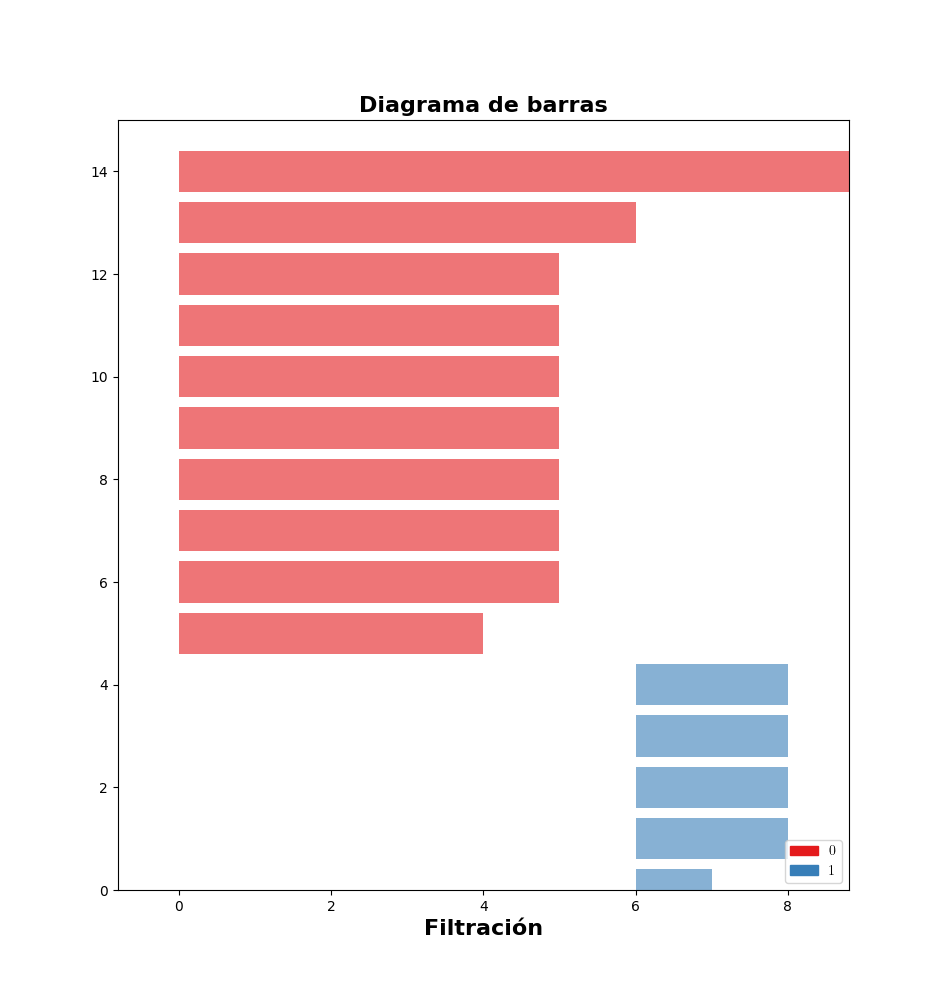
\includegraphics{Images/DiagramaBarrasEj7LOCAL.png}}
					\end{figure}
				\endminipage
				\minipage{0.5\textwidth}
					\begin{figure}[H]
						\resizebox{1.0\textwidth}{!}{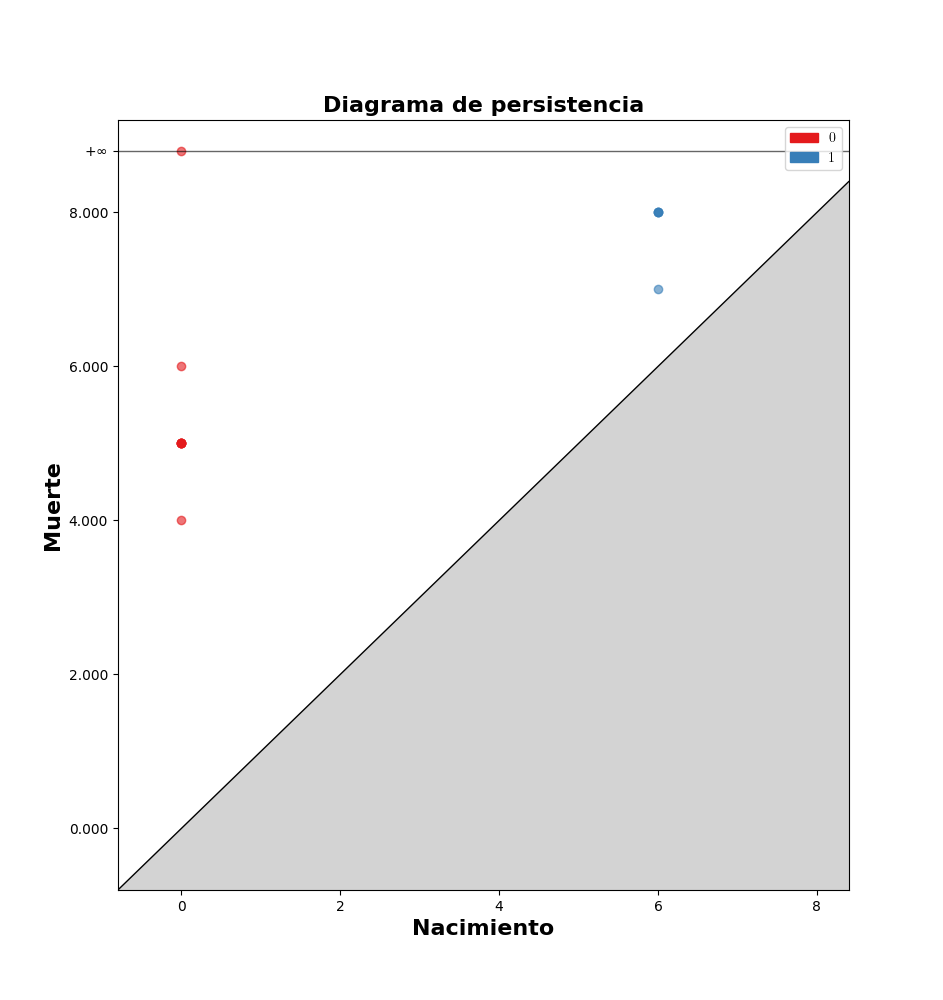
\includegraphics{Images/DiagramaPersistenciaEj7LOCAL.png}}
					\end{figure}
				\endminipage
			\end{figure}
			
			\begin{itemize}
				\item{\textbf{Interpretación global}}
			\end{itemize}
			\begin{figure}[H]
				\fbox{\minipage{0.225\textwidth}
				    	\begin{figure}[H]
						\resizebox{1.0\textwidth}{!}{\begin{tikzpicture}[
							roundnode/.style={circle, draw=black, thick, fill=white, minimum size=7mm},
							]
							%Nodes
							\node           (label) 	at	(1,4) 		{Filtración 0 (t=1.0)};
							\node[roundnode]      (n0) 	at 	(4,1)           {0};
							\node[roundnode]      (n1) 	at 	(4,-1)          {1};
							\node[roundnode]      (n2) 	at 	(2,2)           {2};
							\node[roundnode]      (n3) 	at 	(2,0)           {3};
							\node[roundnode]      (n4)      at 	(2,-2)		{4};
							\node[roundnode]      (n5)      at 	(0,3)		{5};
							\node[roundnode]      (n6)      at 	(0,1)		{6};
							\node[roundnode]      (n7) 	at 	(0,-1)           {7};
							\node[roundnode]      (n8) 	at 	(0,-3)           {8};
							\node[roundnode]      (n9) 	at 	(-2,2)           {9};
							\node[roundnode]      (n10) 	at 	(-2,0)           {10};
							\node[roundnode]      (n11) 	at 	(-2,-2)           {11};
							\node 		(label2) 	at 	(1,-4) 		{$\beta_{0}=10,\beta_{1}=0$};
							
							\begin{pgfonlayer}{background}
							%Lines
							\draw[thick] (n11.mid) --  (n8);
							\draw[thick] (n9.mid) --  (n5);
							\end{pgfonlayer}
						\end{tikzpicture}}	
					\end{figure}	
				\endminipage}
				\fbox{\minipage{0.225\textwidth}
				    	\begin{figure}[H]
						\resizebox{1.0\textwidth}{!}{\begin{tikzpicture}[
							roundnode/.style={circle, draw=black, thick, fill=white, minimum size=7mm},
							]
							%Nodes
							\node           (label) 	at	(1,4) 		{Filtración 4 (t=0.6)};
							\node[roundnode]      (n0) 	at 	(4,1)           {0};
							\node[roundnode]      (n1) 	at 	(4,-1)          {1};
							\node[roundnode]      (n2) 	at 	(2,2)           {2};
							\node[roundnode]      (n3) 	at 	(2,0)           {3};
							\node[roundnode]      (n4)      at 	(2,-2)		{4};
							\node[roundnode]      (n5)      at 	(0,3)		{5};
							\node[roundnode]      (n6)      at 	(0,1)		{6};
							\node[roundnode]      (n7) 	at 	(0,-1)           {7};
							\node[roundnode]      (n8) 	at 	(0,-3)           {8};
							\node[roundnode]      (n9) 	at 	(-2,2)           {9};
							\node[roundnode]      (n10) 	at 	(-2,0)           {10};
							\node[roundnode]      (n11) 	at 	(-2,-2)           {11};
							\node 		(label2) 	at 	(1,-4) 		{$\beta_{0}=9,\beta_{1}=0$};
							
							\begin{pgfonlayer}{background}
							%Lines
							\draw[thick] (n11.mid) --  (n8);
							\draw[thick] (n9.mid) --  (n5);
							\draw[thick] (n6.mid) --  (n2);
							\end{pgfonlayer}
						\end{tikzpicture}}	
					\end{figure}	
				\endminipage}
				\fbox{\minipage{0.225\textwidth}
				    	\begin{figure}[H]
						\resizebox{1.0\textwidth}{!}{\begin{tikzpicture}[
							roundnode/.style={circle, draw=black, thick, fill=white, minimum size=7mm},
							]
							%Nodes
							\node           (label) 	at	(1,4) 		{Filtración 5 (t=0.5)};
							\node[roundnode]      (n0) 	at 	(4,1)           {0};
							\node[roundnode]      (n1) 	at 	(4,-1)          {1};
							\node[roundnode]      (n2) 	at 	(2,2)           {2};
							\node[roundnode]      (n3) 	at 	(2,0)           {3};
							\node[roundnode]      (n4)      at 	(2,-2)		{4};
							\node[roundnode]      (n5)      at 	(0,3)		{5};
							\node[roundnode]      (n6)      at 	(0,1)		{6};
							\node[roundnode]      (n7) 	at 	(0,-1)           {7};
							\node[roundnode]      (n8) 	at 	(0,-3)           {8};
							\node[roundnode]      (n9) 	at 	(-2,2)           {9};
							\node[roundnode]      (n10) 	at 	(-2,0)           {10};
							\node[roundnode]      (n11) 	at 	(-2,-2)           {11};
							\node 		(label2) 	at 	(1,-4) 		{$\beta_{0}=2,\beta_{1}=0$};
							
							\begin{pgfonlayer}{background}
							%Lines
							\draw[thick] (n11.mid) --  (n8);
							\draw[thick] (n9.mid) --  (n5);
							\draw[thick] (n6.mid) --  (n2);
							\draw[thick] (n10.mid) --  (n7);
							\draw[thick] (n10.mid) --  (n6);
							\draw[thick] (n9.mid) --  (n6);
							\draw[thick] (n7.mid) --  (n4);
							\draw[thick] (n6.mid) --  (n3);
							\draw[thick] (n3.mid) --  (n1);
							\draw[thick] (n2.mid) --  (n0);
							\end{pgfonlayer}
						\end{tikzpicture}}	
					\end{figure}	
				\endminipage}
				\fbox{\minipage{0.225\textwidth}
				    	\begin{figure}[H]
						\resizebox{1.0\textwidth}{!}{\begin{tikzpicture}[
							roundnode/.style={circle, draw=black, fill=white, thick, minimum size=7mm},
							]
							%Nodes
							\node           (label) 	at	(1,4) 		{Filtración 6 (t=0.4)};
							\node[roundnode]      (n0) 	at 	(4,1)           {0};
							\node[roundnode]      (n1) 	at 	(4,-1)          {1};
							\node[roundnode]      (n2) 	at 	(2,2)           {2};
							\node[roundnode]      (n3) 	at 	(2,0)           {3};
							\node[roundnode]      (n4)      at 	(2,-2)		{4};
							\node[roundnode]      (n5)      at 	(0,3)		{5};
							\node[roundnode]      (n6)      at 	(0,1)		{6};
							\node[roundnode]      (n7) 	at 	(0,-1)           {7};
							\node[roundnode]      (n8) 	at 	(0,-3)           {8};
							\node[roundnode]      (n9) 	at 	(-2,2)           {9};
							\node[roundnode]      (n10) 	at 	(-2,0)           {10};
							\node[roundnode]      (n11) 	at 	(-2,-2)           {11};
							\node 		(label2) 	at 	(1,-4) 		{$\beta_{0}=1,\beta_{1}=3$};
							
							\begin{pgfonlayer}{background}
						
							\fill[fill=black!20,opacity=1] (n11.mid) -- (n8.mid) -- (n4.mid) -- cycle;
							\fill[fill=black!20,opacity=1] (n11.mid) -- (n7.mid) -- (n4.mid) -- cycle;
							\fill[fill=black!20,opacity=1] (n9.mid) -- (n6.mid) -- (n2.mid) -- cycle;
							\fill[fill=black!20,opacity=1] (n9.mid) -- (n5.mid) -- (n2.mid) -- cycle;
							
							\draw[thick] (n11.mid) --  (n8.mid);
							\draw[thick] (n11.mid) --  (n7.mid);
							\draw[thick] (n11.mid) --  (n4.mid);
							\draw[thick] (n10.mid) --  (n7.mid);
							\draw[thick] (n10.mid) --  (n6);
							\draw[thick] (n9.mid) --  (n6.mid);
							\draw[thick] (n9.mid) --  (n5.mid);
							\draw[thick] (n9.mid) --  (n2.mid);
							\draw[thick] (n8.mid) --  (n4);
							\draw[thick] (n7.mid) --  (n4);
							\draw[thick] (n7.mid) --  (n3);
							\draw[thick] (n6.mid) --  (n3);
							\draw[thick] (n6.mid) --  (n2);
							\draw[thick] (n5.mid) --  (n2);
							\draw[thick] (n4.mid) --  (n1);
							\draw[thick] (n3.mid) --  (n1);
							\draw[thick] (n3.mid) --  (n0);
							\draw[thick] (n2.mid) --  (n0);
							
							\end{pgfonlayer}
						\end{tikzpicture}}	
					\end{figure}	
				\endminipage}
    			\end{figure}
			\begin{figure}[H]
				\fbox{\minipage{0.225\textwidth}
				    	\begin{figure}[H]
						\resizebox{1.0\textwidth}{!}{\begin{tikzpicture}[
							roundnode/.style={circle, draw=black, thick, fill=white, minimum size=7mm},
							]
							%Nodes
							\node           (label) 	at	(1,4) 		{Filtración 7 (t=0.3)};
							\node[roundnode]      (n0) 	at 	(4,1)           {0};
							\node[roundnode]      (n1) 	at 	(4,-1)          {1};
							\node[roundnode]      (n2) 	at 	(2,2)           {2};
							\node[roundnode]      (n3) 	at 	(2,0)           {3};
							\node[roundnode]      (n4)      at 	(2,-2)		{4};
							\node[roundnode]      (n5)      at 	(0,3)		{5};
							\node[roundnode]      (n6)      at 	(0,1)		{6};
							\node[roundnode]      (n7) 	at 	(0,-1)           {7};
							\node[roundnode]      (n8) 	at 	(0,-3)           {8};
							\node[roundnode]      (n9) 	at 	(-2,2)           {9};
							\node[roundnode]      (n10) 	at 	(-2,0)           {10};
							\node[roundnode]      (n11) 	at 	(-2,-2)           {11};
							\node 		(label2) 	at 	(1,-4) 		{$\beta_{0}=1,\beta_{1}=2$};
							
							\begin{pgfonlayer}{background}							
						

							\fill[fill=black!20,opacity=1] (n11.mid) -- (n8.mid) -- (n4.mid) -- cycle;
							\fill[fill=black!20,opacity=1] (n11.mid) -- (n7.mid) -- (n4.mid) -- cycle;
							\fill[fill=black!20,opacity=1] (n10.mid) to[bend right] (n4.mid) -- (n7.mid) -- cycle;
							\fill[fill=black!20,opacity=1] (n10.mid) to[bend left] (n2.mid) -- (n6.mid) -- cycle;
							\fill[fill=black!20,opacity=1] (n9.mid) -- (n6.mid) -- (n2.mid) -- cycle;
							\fill[fill=black!20,opacity=1] (n9.mid) -- (n5.mid) -- (n2.mid) -- cycle;
							\fill[fill=black!20,opacity=1] (n6.mid) to[bend left] (n1.mid) -- (n3.mid) -- cycle;
							\fill[fill=black!20,opacity=1] (n6.mid) -- (n3.mid) -- (n0.mid) -- cycle;
							\fill[fill=black!20,opacity=1] (n6.mid) -- (n2.mid) -- (n0.mid) -- cycle;
							
							\draw[thick] (n11.mid) --  (n8);
							\draw[thick] (n11.mid) --  (n7);
							\draw[thick] (n11.mid) --  (n4.mid);
							\draw[thick] (n10.mid) --  (n7);
							\draw[thick] (n10.mid) --  (n6);
							\draw[thick] (n9.mid) --  (n6);
							\draw[thick] (n9.mid) --  (n5);
							\draw[thick] (n9.mid) --  (n2.mid);
							\draw[thick] (n8.mid) --  (n4);
							\draw[thick] (n7.mid) --  (n4);
							\draw[thick] (n7.mid) --  (n3);
							\draw[thick] (n6.mid) --  (n3);
							\draw[thick] (n6.mid) --  (n2);
							\draw[thick] (n6.mid) --  (n0);
							\draw[thick] (n5.mid) --  (n2);
							\draw[thick] (n4.mid) --  (n1);
							\draw[thick] (n3.mid) --  (n1);
							\draw[thick] (n3.mid) --  (n0);
							\draw[thick] (n2.mid) --  (n0);
							\end{pgfonlayer}
						\end{tikzpicture}}	
					\end{figure}	
				\endminipage}
				\fbox{\minipage{0.225\textwidth}
				    	\begin{figure}[H]
						\resizebox{1.0\textwidth}{!}{\begin{tikzpicture}[
							roundnode/.style={circle, draw=black, thick, fill=white, minimum size=7mm},
							]
							%Nodes
							\node           (label) 	at	(1,4) 		{Filtración 8 (t=0.2)};
							\node[roundnode]      (n0) 	at 	(4,1)           {0};
							\node[roundnode]      (n1) 	at 	(4,-1)          {1};
							\node[roundnode]      (n2) 	at 	(2,2)           {2};
							\node[roundnode]      (n3) 	at 	(2,0)           {3};
							\node[roundnode]      (n4)      at 	(2,-2)		{4};
							\node[roundnode]      (n5)      at 	(0,3)		{5};
							\node[roundnode]      (n6)      at 	(0,1)		{6};
							\node[roundnode]      (n7) 	at 	(0,-1)           {7};
							\node[roundnode]      (n8) 	at 	(0,-3)           {8};
							\node[roundnode]      (n9) 	at 	(-2,2)           {9};
							\node[roundnode]      (n10) 	at 	(-2,0)           {10};
							\node[roundnode]      (n11) 	at 	(-2,-2)           {11};
							\node 		(label2) 	at 	(1,-4) 		{$\beta_{0}=1,\beta_{1}=0$};
							
							\begin{pgfonlayer}{background}							
						

							\fill[fill=black!20,opacity=1] (n11.mid) -- (n8.mid) -- (n4.mid) -- cycle;
							\fill[fill=black!20,opacity=1] (n11.mid) -- (n7.mid) -- (n4.mid) -- cycle;
							\fill[fill=black!20,opacity=1] (n10.mid) to[bend right] (n4.mid) -- (n7.mid) -- cycle;
							\fill[fill=black!20,opacity=1] (n10.mid) -- (n7.mid) -- (n3.mid) -- cycle;
							\fill[fill=black!20,opacity=1] (n10.mid) -- (n6.mid) -- (n3.mid) -- cycle;
							\fill[fill=black!20,opacity=1] (n10.mid) to[bend left] (n2.mid) -- (n6.mid) -- cycle;
							\fill[fill=black!20,opacity=1] (n9.mid) to[bend right] (n3.mid) -- (n6.mid) -- cycle;
							\fill[fill=black!20,opacity=1] (n9.mid) -- (n6.mid) -- (n2.mid) -- cycle;
							\fill[fill=black!20,opacity=1] (n9.mid) -- (n5.mid) -- (n2.mid) -- cycle;
							\fill[fill=black!20,opacity=1] (n7.mid) -- (n4.mid) -- (n1.mid) -- cycle;
							\fill[fill=black!20,opacity=1] (n7.mid) -- (n3.mid) -- (n1.mid) -- cycle;
							\fill[fill=black!20,opacity=1] (n6.mid) to[bend left] (n1.mid) -- (n3.mid) -- cycle;
							\fill[fill=black!20,opacity=1] (n6.mid) -- (n3.mid) -- (n0.mid) -- cycle;
							\fill[fill=black!20,opacity=1] (n6.mid) -- (n2.mid) -- (n0.mid) -- cycle;
							\fill[fill=black!20,opacity=1] (n5.mid) to[bend left] (n0.mid) -- (n2.mid) -- cycle;
							
							\draw[thick] (n11.mid) --  (n8.mid);
							\draw[thick] (n11.mid) --  (n7.mid);
							\draw[thick] (n11.mid) --  (n4.mid);
							\draw[thick] (n10.mid) --  (n7.mid);
							\draw[thick] (n10.mid) --  (n6.mid);
							\draw[thick] (n10.mid) --  (n3.mid);
							\draw[thick] (n9.mid) --  (n6.mid);
							\draw[thick] (n9.mid) --  (n5.mid);
							\draw[thick] (n9.mid) --  (n2.mid);
							\draw[thick] (n8.mid) --  (n4.mid);
							\draw[thick] (n7.mid) --  (n4.mid);
							\draw[thick] (n7.mid) --  (n3.mid);
							\draw[thick] (n7.mid) --  (n1.mid);
							\draw[thick] (n6.mid) --  (n3.mid);
							\draw[thick] (n6.mid) --  (n2.mid);
							\draw[thick] (n6.mid) --  (n0.mid);
							\draw[thick] (n5.mid) --  (n2.mid);
							\draw[thick] (n4.mid) --  (n1.mid);
							\draw[thick] (n3.mid) --  (n1.mid);
							\draw[thick] (n3.mid) --  (n0.mid);
							\draw[thick] (n2.mid) --  (n0.mid);
							\end{pgfonlayer}
						\end{tikzpicture}}	
					\end{figure}	
				\endminipage}
				\fbox{\minipage{0.225\textwidth}
				    	\begin{figure}[H]
						\resizebox{1.0\textwidth}{!}{\begin{tikzpicture}[
							roundnode/.style={circle, draw=black, thick, fill=white, minimum size=7mm},
							]
							%Nodes
							\node           (label) 	at	(1,4) 		{Filtración 9 (t=0.1)};
							\node[roundnode]      (n0) 	at 	(4,1)           {0};
							\node[roundnode]      (n1) 	at 	(4,-1)          {1};
							\node[roundnode]      (n2) 	at 	(2,2)           {2};
							\node[roundnode]      (n3) 	at 	(2,0)           {3};
							\node[roundnode]      (n4)      at 	(2,-2)		{4};
							\node[roundnode]      (n5)      at 	(0,3)		{5};
							\node[roundnode]      (n6)      at 	(0,1)		{6};
							\node[roundnode]      (n7) 	at 	(0,-1)           {7};
							\node[roundnode]      (n8) 	at 	(0,-3)           {8};
							\node[roundnode]      (n9) 	at 	(-2,2)           {9};
							\node[roundnode]      (n10) 	at 	(-2,0)           {10};
							\node[roundnode]      (n11) 	at 	(-2,-2)           {11};
							\node 		(label2) 	at 	(1,-4) 		{$\beta_{0}=1,\beta_{1}=0$};
							
							\begin{pgfonlayer}{background}							
						

							\fill[fill=black!20,opacity=1] (n11.mid) -- (n8.mid) -- (n4.mid) -- cycle;
							\fill[fill=black!20,opacity=1] (n11.mid) -- (n7.mid) -- (n4.mid) -- cycle;
							\fill[fill=black!20,opacity=1] (n11.mid) to[bend left] (n3.mid) -- (n7.mid) -- cycle;
							\fill[fill=black!20,opacity=1] (n10.mid) to[bend right] (n4.mid) -- (n7.mid) -- cycle;
							\fill[fill=black!20,opacity=1] (n10.mid) -- (n7.mid) -- (n3.mid) -- cycle;
							\fill[fill=black!20,opacity=1] (n10.mid) -- (n6.mid) -- (n3.mid) -- cycle;
							\fill[fill=black!20,opacity=1] (n10.mid) to[bend left] (n2.mid) -- (n6.mid) -- cycle;
							\fill[fill=black!20,opacity=1] (n9.mid) to[bend right] (n3.mid) -- (n6.mid) -- cycle;
							\fill[fill=black!20,opacity=1] (n9.mid) -- (n6.mid) -- (n2.mid) -- cycle;
							\fill[fill=black!20,opacity=1] (n9.mid) -- (n5.mid) -- (n2.mid) -- cycle;
							\fill[fill=black!20,opacity=1] (n8.mid) to[bend right] (n1.mid) -- (n4.mid) -- cycle;
							\fill[fill=black!20,opacity=1] (n7.mid) -- (n4.mid) -- (n1.mid) -- cycle;
							\fill[fill=black!20,opacity=1] (n7.mid) -- (n3.mid) -- (n1.mid) -- cycle;
							\fill[fill=black!20,opacity=1] (n7.mid) to[bend right] (n0.mid) -- (n3.mid) -- cycle;
							\fill[fill=black!20,opacity=1] (n6.mid) to[bend left] (n1.mid) -- (n3.mid) -- cycle;
							\fill[fill=black!20,opacity=1] (n6.mid) -- (n3.mid) -- (n0.mid) -- cycle;
							\fill[fill=black!20,opacity=1] (n6.mid) -- (n2.mid) -- (n0.mid) -- cycle;
							\fill[fill=black!20,opacity=1] (n5.mid) to[bend left] (n0.mid) -- (n2.mid) -- cycle;
							
							\draw[thick] (n11.mid) --  (n8.mid);
							\draw[thick] (n11.mid) --  (n7.mid);
							\draw[thick] (n11.mid) --  (n4.mid);
							\draw[thick] (n10.mid) --  (n7.mid);
							\draw[thick] (n10.mid) --  (n6.mid);
							\draw[thick] (n10.mid) --  (n3.mid);
							\draw[thick] (n9.mid) --  (n6.mid);
							\draw[thick] (n9.mid) --  (n5.mid);
							\draw[thick] (n9.mid) --  (n2.mid);
							\draw[thick] (n8.mid) --  (n4.mid);
							\draw[thick] (n7.mid) --  (n4.mid);
							\draw[thick] (n7.mid) --  (n3.mid);
							\draw[thick] (n7.mid) --  (n1.mid);
							\draw[thick] (n6.mid) --  (n3.mid);
							\draw[thick] (n6.mid) --  (n2.mid);
							\draw[thick] (n6.mid) --  (n0.mid);
							\draw[thick] (n5.mid) --  (n2.mid);
							\draw[thick] (n4.mid) --  (n1.mid);
							\draw[thick] (n3.mid) --  (n1.mid);
							\draw[thick] (n3.mid) --  (n0.mid);
							\draw[thick] (n2.mid) --  (n0.mid);
							\end{pgfonlayer}
						\end{tikzpicture}}	
					\end{figure}	
				\endminipage}
				\fbox{\minipage{0.225\textwidth}
				    	\begin{figure}[H]
						\resizebox{1.0\textwidth}{!}{\begin{tikzpicture}[
							roundnode/.style={circle, draw=black, thick, fill=white, minimum size=7mm},
							]
							%Nodes
							\node           (label) 	at	(1,4) 		{Filtración 10 (t=0.0)};
							\node[roundnode]      (n0) 	at 	(4,1)           {0};
							\node[roundnode]      (n1) 	at 	(4,-1)          {1};
							\node[roundnode]      (n2) 	at 	(2,2)           {2};
							\node[roundnode]      (n3) 	at 	(2,0)           {3};
							\node[roundnode]      (n4)      at 	(2,-2)		{4};
							\node[roundnode]      (n5)      at 	(0,3)		{5};
							\node[roundnode]      (n6)      at 	(0,1)		{6};
							\node[roundnode]      (n7) 	at 	(0,-1)           {7};
							\node[roundnode]      (n8) 	at 	(0,-3)           {8};
							\node[roundnode]      (n9) 	at 	(-2,2)           {9};
							\node[roundnode]      (n10) 	at 	(-2,0)           {10};
							\node[roundnode]      (n11) 	at 	(-2,-2)           {11};
							\node 		(label2) 	at 	(1,-4) 		{$\beta_{0}=1,\beta_{1}=0$};
							
							\begin{pgfonlayer}{background}							
						

							\fill[fill=black!20,opacity=1] (n11.mid) -- (n8.mid) -- (n4.mid) -- cycle;
							\fill[fill=black!20,opacity=1] (n11.mid) -- (n7.mid) -- (n4.mid) -- cycle;
							\fill[fill=black!20,opacity=1] (n11.mid) to[bend left] (n3.mid) -- (n7.mid) -- cycle;
							\fill[fill=black!20,opacity=1] (n10.mid) to[bend right] (n4.mid) -- (n7.mid) -- cycle;
							\fill[fill=black!20,opacity=1] (n10.mid) -- (n7.mid) -- (n3.mid) -- cycle;
							\fill[fill=black!20,opacity=1] (n10.mid) -- (n6.mid) -- (n3.mid) -- cycle;
							\fill[fill=black!20,opacity=1] (n10.mid) to[bend left] (n2.mid) -- (n6.mid) -- cycle;
							\fill[fill=black!20,opacity=1] (n9.mid) to[bend right] (n3.mid) -- (n6.mid) -- cycle;
							\fill[fill=black!20,opacity=1] (n9.mid) -- (n6.mid) -- (n2.mid) -- cycle;
							\fill[fill=black!20,opacity=1] (n9.mid) -- (n5.mid) -- (n2.mid) -- cycle;
							\fill[fill=black!20,opacity=1] (n8.mid) to[bend right] (n1.mid) -- (n4.mid) -- cycle;
							\fill[fill=black!20,opacity=1] (n7.mid) -- (n4.mid) -- (n1.mid) -- cycle;
							\fill[fill=black!20,opacity=1] (n7.mid) -- (n3.mid) -- (n1.mid) -- cycle;
							\fill[fill=black!20,opacity=1] (n7.mid) to[bend right] (n0.mid) -- (n3.mid) -- cycle;
							\fill[fill=black!20,opacity=1] (n6.mid) to[bend left] (n1.mid) -- (n3.mid) -- cycle;
							\fill[fill=black!20,opacity=1] (n6.mid) -- (n3.mid) -- (n0.mid) -- cycle;
							\fill[fill=black!20,opacity=1] (n6.mid) -- (n2.mid) -- (n0.mid) -- cycle;
							\fill[fill=black!20,opacity=1] (n5.mid) to[bend left] (n0.mid) -- (n2.mid) -- cycle;
							
							\draw[thick] (n11.mid) --  (n8.mid);
							\draw[thick] (n11.mid) --  (n7.mid);
							\draw[thick] (n11.mid) --  (n4.mid);
							\draw[thick] (n10.mid) --  (n7.mid);
							\draw[thick] (n10.mid) --  (n6.mid);
							\draw[thick] (n10.mid) --  (n3.mid);
							\draw[thick] (n9.mid) --  (n6.mid);
							\draw[thick] (n9.mid) --  (n5.mid);
							\draw[thick] (n9.mid) --  (n2.mid);
							\draw[thick] (n8.mid) --  (n4.mid);
							\draw[thick] (n7.mid) --  (n4.mid);
							\draw[thick] (n7.mid) --  (n3.mid);
							\draw[thick] (n7.mid) --  (n1.mid);
							\draw[thick] (n6.mid) --  (n3.mid);
							\draw[thick] (n6.mid) --  (n2.mid);
							\draw[thick] (n6.mid) --  (n0.mid);
							\draw[thick] (n5.mid) --  (n2.mid);
							\draw[thick] (n4.mid) --  (n1.mid);
							\draw[thick] (n3.mid) --  (n1.mid);
							\draw[thick] (n3.mid) --  (n0.mid);
							\draw[thick] (n2.mid) --  (n0.mid);
							\end{pgfonlayer}
						\end{tikzpicture}}	
					\end{figure}	
				\endminipage}
    			\end{figure}
			\begin{figure}[H]
				\minipage{0.5\textwidth}
					\begin{figure}[H]
						\resizebox{1.0\textwidth}{!}{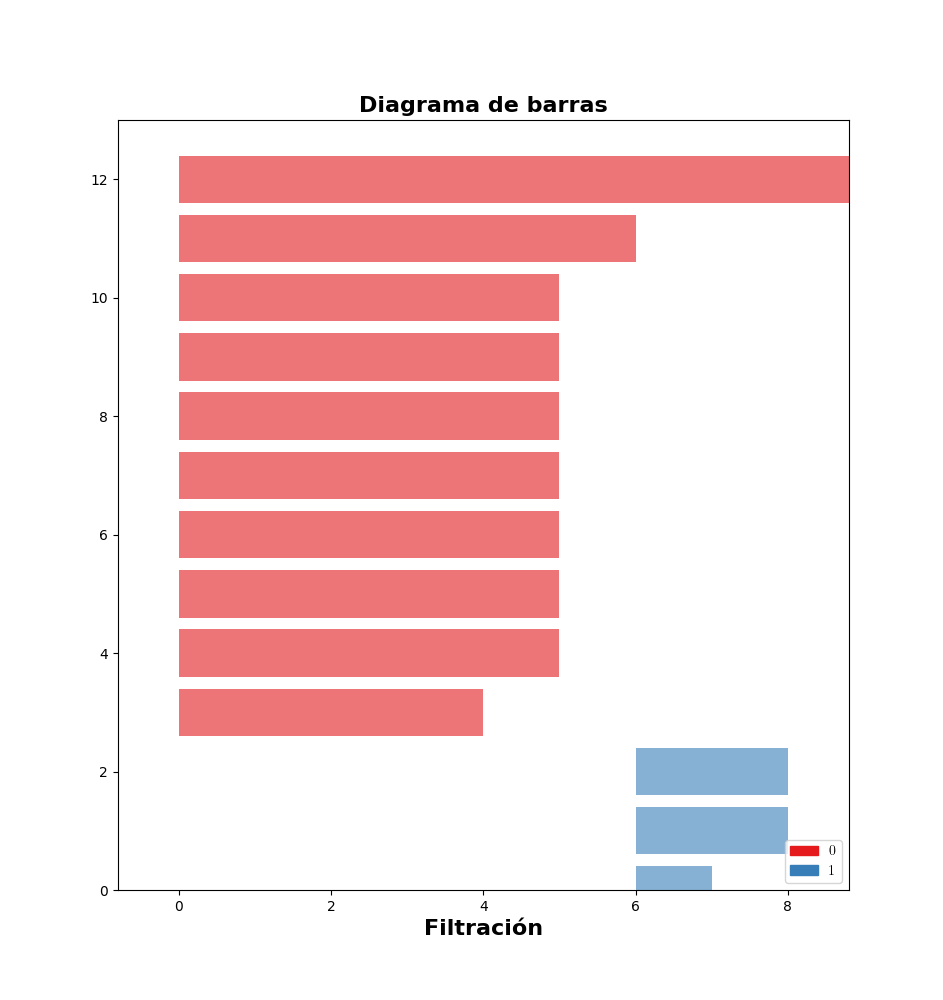
\includegraphics{Images/DiagramaBarrasEj7GLOBAL.png}}
					\end{figure}
				\endminipage
				\minipage{0.5\textwidth}
					\begin{figure}[H]
						\resizebox{1.0\textwidth}{!}{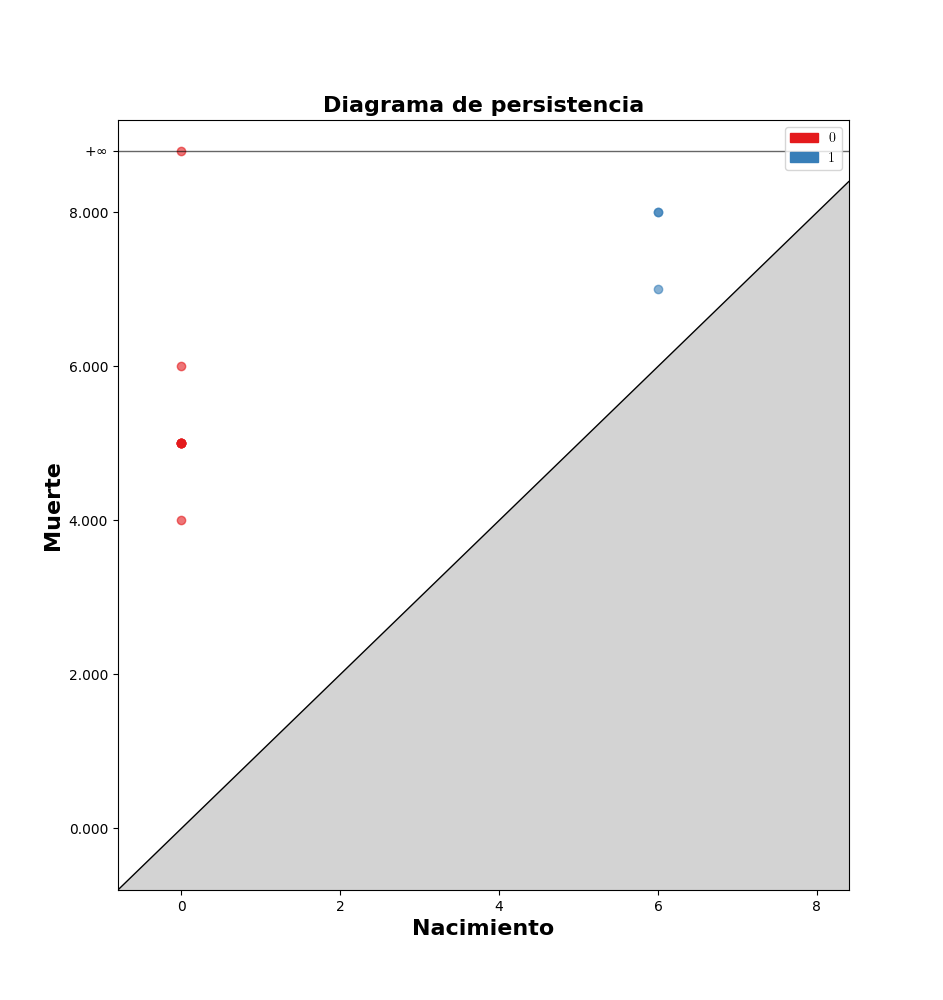
\includegraphics{Images/DiagramaPersistenciaEj7GLOBAL.png}}
					\end{figure}
				\endminipage
			\end{figure}
			\begin{remark}
				Para una mayor claridad, en los dibujos de las filtraciones se han omitido algunas aristas.
			\end{remark}
		\end{ejem}	
		Del ejemplo anterior podemos extraer unas conclusiones muy importantes. Por una parte, observamos que si las neuronas de entrada se conectan
		directamente a las de salida, el conocimiento de la red será ``pobre" ya que será equivalente a la detección de patrones. Por otra parte,
		el incremento del número de Betti $\beta_{1}$ indica que la red determina la neurona de llegada por combinación de las neuronas de salida. De este modo,
		podemos suponer que el aumento de $\beta_{1}$ releja la complejidad del conocimiento adquirido por la red. Por lo tanto, mediante el uso de la homología persistente
		seremos capaces de medir la complejidad del conocimiento adquirido por la red.
	
	\section{Experimentos}
		(En construcción.)
\end{document} 
